%!TeX root = Thesis_LP.tex
% \sisetup{
% list-final-separator= { and },    % Place "et" à la fin de la liste
% range-phrase= { to }             % Place "à" à entre la gamm
% }
\pagestyle{fancy}
\fancyhf{}
\renewcommand{\headrulewidth}{0pt}
\fancyhead[LO]{\emph{Article 1. VSP modeling for \ce{CO2} monitoring}}
\fancyhead[RO]{\thepage}
\fancyhead[LE]{\thepage}

\chapter{Sensitivity of vertical seismic profiling for monitoring
\texorpdfstring{\ce{CO2}}{CO2} storage in a low porosity reservoir - An example
from the St-Lawrence Lowlands, Canada}

\label{ch:article1}
\selectlanguage{english}

\chaptermark{Sensintivity of VSP for \ce{CO2} monitoring} % Titre court
% apparaissant dans l'entête des pages

{\setlength{\parindent}{0cm}
\underline{\textbf{Titre traduit}}\\
Sensibilité du profilage sismique vertical pour la surveillance du  \ce{CO2}
stocké dans un réservoir peu poreux - Exemple des Basses Terres du St Laurent,
Canada

\underline{\textbf{Auteurs}}\\
Lorenzo Perozzi$^1$, Bernard Giroux$^1$, Douglas R. Schmitt$^2$, Randolf S.
Kofman$^2$\\
$^1$ Institut national de la recherche scientifique - Centre Eau Terre
Environnement, 490, de la Couronne, Qu\'ebec, QC, G1K 9A9, CANADA\\
$^2$ Department of Physics, Institute for Geophysical Research, CCIS 4-183,
University of Alberta, Edmonton, AB, T6G 2E1, CANADA

\newpage
\underline{\textbf{Contribution}}
{\setstretch{1.0}
\begin{description}[leftmargin=!,labelwidth=\widthof{\bfseries Randolf S.
Kofman}]
  \setlength\itemsep{0.7em}
  \item[Lorenzo Perozzi] Conceptualisé et réalisé (les mesures de laboratoire,
la modélisation sismique, l’interprétation des résultats) l’étude et rédigé
l’article
  \item[Bernard Giroux]  Conceptualisé l'étude, fourni des conseils sur
l’interprétation des résultats et contribué à la rédaction de l’article.
  \item[Douglas R. Schmitt]  Contribué à la rédaction de l’article
  \item[Randolf S. Kofman]  Fourni de conseils et realisé une partie de mesures
de laboratoire.\\
\end{description}
}


\underline{\textbf{Publication ciblée}}\\
{\setstretch{0.5}
International Journal of Greenhouse Gas Control\\
Première soumission: 6 janvier 2015\\
Soumission après révision: 26 juillet 2015
}


\underline{\textbf{Résumé traduit}}\\
Nous avons réalisé une série de mesures sismiques de laboratoire sous
differentes conditions de pressions et temperature afin de tester la réponse
sismique sur deux échantillons saturés en \ce{CO2} provenant du reservoir des
Basses Terre du Saint Laurent. Les resultats ont montré que la vitesse et
l'amplitude du signal sismique peuvent être utilisées pour detecter le changement
de phase du \ce{CO2}. Les resultats ont aussi servi a calibrer un modèle
géologique héterogène à partir duquel des séismogrammes de profilage sismique vertical ont été générés. Le degré de saturation  autour d'un puits
d'injection a été calculé pour un periode de  \num{50} ans qui inclut
un periode d'injection de \num{15} ans suivie par \num{35} de migration de
\ce{CO2}. Des seismogrammes synthetiques de profilage sismique vertical dans le
temps ont été générés après 5, 15 et 50 ans d'injection. Les resultats ont montré que le
remplacement de la saumure par le \ce{CO2} provoque un délai en temps des
reflecteurs situés au-dessous du reservoir, malgrés ses faibles porosités et
perméabilités. La comparaison entre un modèle homogène classique et le modèle
hétérogène proposé dans ce travail montre que le modèle homogène classique
pourrait conduire à une mauvaise interpretation de l'effet du \ce{CO2} sur la
réponse sismique.
}

\section{Abstract}
We have performed a series of rock physics measurements under various simulated
confining and pore pressure and temperature states to test the seismic response
of two low permeability reservoir samples of the St.\ Lawrence Lowlands
sedimentary basin to different \ce{CO2} phases. Results show that the seismic
velocity and amplitude can be used to detect the \ce{CO2} phase transition. The
laboratory measurements calibrated a heterogeneous geological model from which
synthetic vertical seismic profile (VSP) seismograms were generated. The
saturation states around a single injection point in the geological model were
calculated over a \num{50} year time period which included constant rate
injection for the first \num{15} years followed by \num{35} years of \ce{CO2}
migration. Synthetic time-lapse VSP seismograms were produced after
\numlist{5;15;50} years from the start of injection. Results show that
substitution of brine by \ce{CO2} delays the times of seismic reflection events
below the target reservoir despite its low reservoir permeabilities and
porosities. A comparison between a classical blocky model and our heterogeneous
model shows that the blocky model leads to a misinterpretation of the \ce{CO2}
effects on the seismic response.
\section{Introduction}
The measurement, monitoring and verification (MMV) of geological \ce{CO2}
storage is essential for ensuring storage integrity and social acceptance of
Carbon Capture and Storage (CCS). Satisfying these societal requirements is
necessary to allow the deployment of the MMV technologies at a scale sufficient
to reduce the rate of increase of anthropogenically produced \ce{CO2}. Also, in
a carbon market context, appraisal and verification of stored \ce{CO2} should be
integrated components of CCS projects. As such, monitoring programs of \ce{CO2}
injection should ultimately allow for the quantitative estimation of \ce{CO2}
saturation throughout the reservoir and watch for any migration of carbon
dioxide into surrounding geological formations. Geophysical methods are
challenged in this respect, and multi-method approaches should be favored.
Gravity monitoring can be helpful for mass balance estimation, especially if
downhole gravimeters can be positioned close to the reservoir \citep{dodds13}.
Electrical methods can also play an important role due to the very low
sensitivity of electrical properties to pressure effects and high sensitivity to
pore fluid conductivity \citep{schon04,SchmidtHattenberger2013}. \\
To date, active source seismic methods remain the principal geophysical method
of all monitoring programs. Indeed, seismic methods were shown to be efficient
for MMV due to their high resolution and their sensitivity to porosity and fluid
saturation \citep{White2013a,Lumley2010a,Lumley2010,Carcione2006}.
Nevertheless, there can be a great deal of ambiguity in the quantitative
interpretation of observed seismic responses. Proper interpretation requires
that workers understand how seismic reflectivity will evolve with changes in the
effective stress, temperature, and state of saturation within the subsurface.
Despite these issues it is likely that active-source seismic methods will always
play a central part in \ce{CO2} monitoring programs due to their high resolution
compared to other geophysical methods. Consequently responsible operators will
need to properly understand the effects of \ce{CO2} on seismic properties. \\
% Since \num{2008}, the INRS \ce{CO2} research chair granted by the Minist\`ere
% du D\'e\-ve\-loppe\-ment durable, de l'Environnement et des Parcs du Qu\'ebec,
% studies the feasibility of geological storage of \ce{CO2} in the province of
% Quebec, Canada.  As part of the research program of the Chair, an assessment of
% the performance of seismic monitoring is carried out for in the particular
% context of the St.\ Lawrence Lowlands.\\
The Cambrian-Ordovician sedimentary basin of the St.\ Lawrence Platform in
southern Quebec, Canada, has been identified as the most prospective basin for
\ce{CO2} storage in the province \citep{Malo2012}. The Bécancour region is
located on the south shore of the St.\ Lawrence River, midway between Montreal
and Quebec City (\Cref{fig:map}). The Bé\-can\-cour region's deep saline
aquifers were selected as a potential target for injection of \ce{CO2} in a
future pilot project. This selection was based on seismic reflection and well
log data available from gas exploration, and based on the proximity of an
industrial zone emitting up to \SI{1}{\mega\tonne} of \ce{CO2} per year. The
success of the storage depends on the capability to monitor movements of the
injected gas into the subsurface. As in all current CCS projects, seismic
methods are an important component of the monitoring program at Bécancour. In
such projects, prior estimation of elastic property changes in response to the
injection of \ce{CO2} is crucial to perform proper monitoring and subsequent
interpretation of the time-lapse seismic data. There is thus a mandatory need to
understand how injected \ce{CO2} influences seismic response and how seismic
methods could obtain reliable quantitative estimates of injected \ce{CO2}
\citep{White2013}.\\
\begin{figure}[!ht]
        \centering
        \begin{subfigure}[b]{.55\textwidth}
                \caption{Distribution of sedimentary basins on the south shore
of the St. Lawrence River. Bottom right inset is the distribution of deep saline
aquifers in Canada \citep{Wright2013}.}
                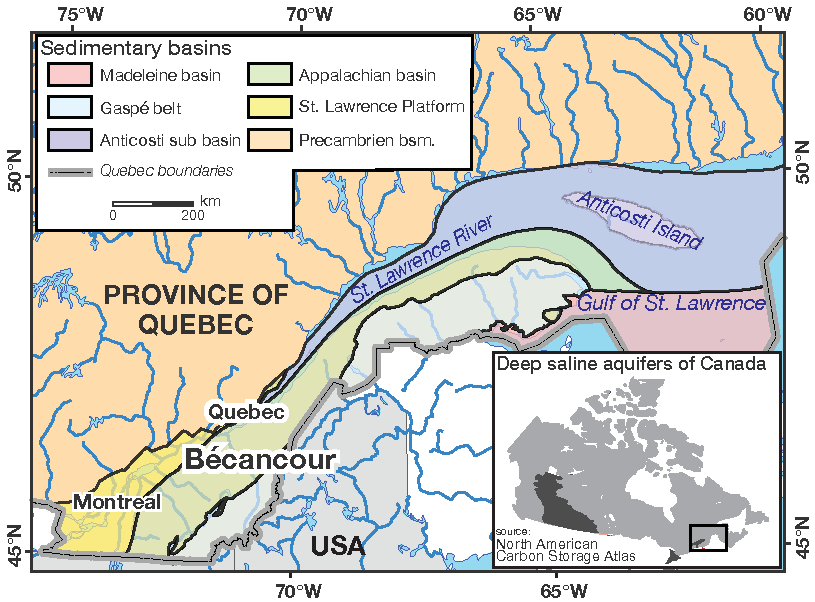
\includegraphics[width=\textwidth]{fig/map.pdf}
                \label{fig:map}
        \end{subfigure}%

        \begin{subfigure}[b]{.55\textwidth}
                \caption{Simplified stratigraphy of the St. Lawrence Platform.}
                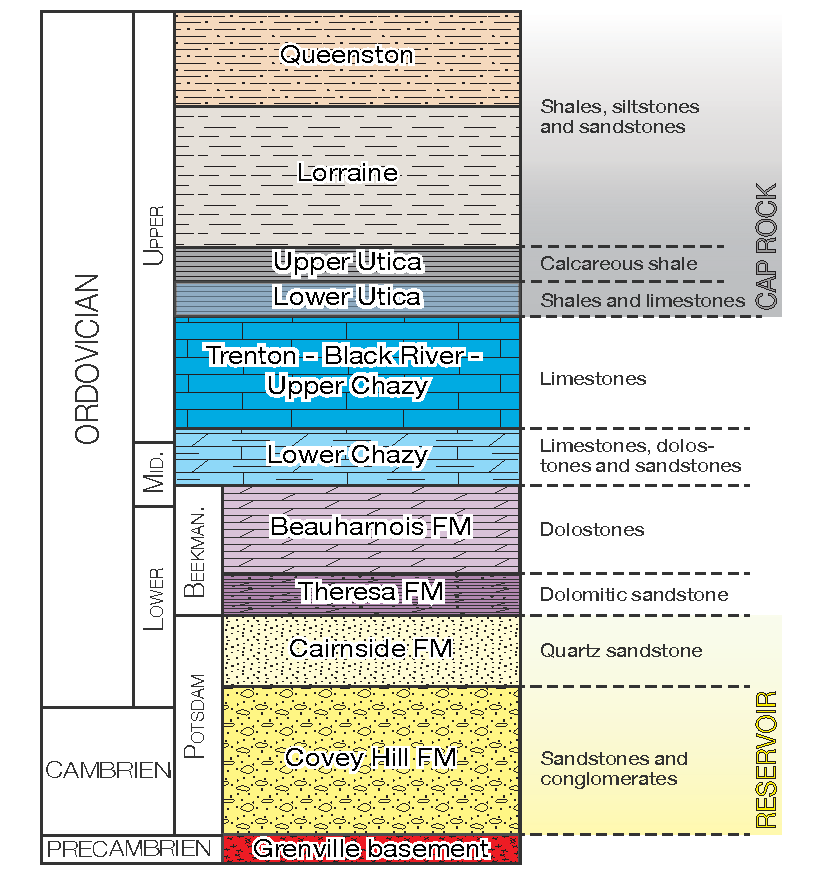
\includegraphics[width=\textwidth]{fig/strati.pdf}
                \label{fig:strati}
        \end{subfigure}

        \caption{Geographical and stratigraphical map of the studied area.
Modified from \citep{Malo2012} and  \citep{Claprood2012}}
        \label{fig:geo}.
\end{figure}
The aim of this study is to better understand the dependence of the seismic
properties on the porosity, mineralogy and pore fluids found in the
Bé\-can\-cour reservoir through both laboratory measurements and numerical
modeling.  In this contribution, we first present a set of laboratory
measurements of the compressional ($P$) and shear ($S$) wave velocity and
amplitude made on two sandstone samples from the target reservoir, fully
saturated with \ce{CO2} at different temperatures and pressures. The results of
these experiments are then used to build a geological model and generate
synthetic seismograms forecasting the response to \ce{CO2} injection in the
reservoir formations.
\section{Bécancour reservoir properties}
The St.\ Lawrence Lowlands sedimentary basin is located between the Precambrian
Grenville basement in the north-west and the Appalachian thrust domain in the
south-east (\Cref{fig:map}). The Paleozoic sedimentary succession of the St.\
Lawrence Platform is shown in \cref{fig:strati}. The Potsdam Group lies
unconformably upon the metamorphic Precambrian Grenville basement. It is
comprised of the Covey Hill (Cambrian sandstones and conglomerates) and the
Cairnside (lower Ordovician quartz sandstone) formations. The remainder of the
section is all of Ordovician age. The Beekmantown Group includes the Theresa
(dolomitic sandstones) and the Beau\-har\-nois (dolostones) formations. The
lower Chazy unit is composed of limestones, dolostones, and sandstones. The
Trenton, Black River, and upper Chazy groups, are limestones. The Trenton Group
is overlain by the Utica Shale and several hundred meters of interbedded shales,
siltstones and sandstones of the Lorraine Group. The lower Utica Shale comprises
limestone beds and is more calcareous than the upper Utica Shale. Deep saline
aquifers are found in the Trenton, Beekmantown and Potsdam Groups.\\
The Covey Hill sandstone (lower Potsdam) appears as the most suitable saline
aquifer for \ce{CO2} injection/storage. This unit has the largest injectable
pore volume due to highest porosity (\SI{6}{\percent}), net pay thickness
(\SI{196}{\metre}), highest matrix permeability (\SI{2.4e-16}{\metre\squared})
and lowest salinity (\SI[per-mode=symbol]{108.500}{\milli\gram\per\litre}) that
may assure feasible injectivity.
The sandstones of the Covey Hill formation are located at depths of
\SIrange{1100}{1400}{\metre} where injected \ce{CO2} would be in a supercritical
state that has lower density and viscosity than the liquid brine it displaces.\\
The \ce{CO2} can also be injected in the Cairnside (upper Potsdam), however its
lower permeability, lower porosity and more saline waters are less favorable for
the storage of \ce{CO2} \citep{TranNgoc2014}. Moreover, the temperature gradient
of Bé\-can\-cour reservoir (\SI[multi-part-units =
single]{23.5(6)}{\degreeCelsius\per\km}) may not lead to a supercritical state
of \ce{CO2} everywhere in the Cairnside Formation, due to the shallower depth of
its formation top \citep{Claprood2012}.\\
The regional caprock unit consists of the Utica and Lorraine shales. The
thickness (\SI{>800}{\metre}) and permeability (\SI{1e-19}{\metre\squared}) of
the caprock units in the Bé\-can\-cour region are apparently capable of
preventing buoyancy-driven migration of injected \ce{CO2} to the surface, as
they have maintained over-pressured conditions in the saline aquifers
\citep{TranNgoc2014}. Petrophysical and hydrogeological properties of the
reservoir are summarized in Table~\cref{tbl:prop}.
\begin{table}[tpb]
	\caption{Physical properties of the Potsdam group reservoir and the
Utica/Lorraine cap-rock.}
	\label{tbl:prop}
	\sisetup{per-mode = symbol,table-format = 1.2e-2}
    \centering
    \begin{threeparttable}[b]
        \begin{tabular}{ll@{\hspace{2em}}
        S[table-comparator = true,table-format = 1.0e-2]
        @{\hspace{3em}}
        S
        @{\hspace{3em}}
        S[table-format = 1.1e-2]
        }
            \toprule
            &&  & \multicolumn{2}{c}{Potsdam Group}\\
            \cmidrule(r){4-5}
             && {Cap Rock} & {Cairnside} & {Covey Hill} \\
	        % \cmidrule(r){3-5}
            \midrule
	        {Lithology} && {shale}  & {sandstone} & {sandstone} \\
			Grain density& (\si{\gram\per\cubic\cm)}  & {2.700} & {2.632} & {2.613} \\
			Porosity\tnote{a}&  (\si{\percent}) & {4} & {3.35} & {6}      \\
			Matrix permeability\tnote{b}& (\si{\metre\squared}) & 4e-19& 1.2e-16
&2.5e-4\\
			Horizontal permeability\tnote{a}& (\si{\metre\squared}) & n/a & 8.89e-15 &
8.9e-16\\
			Vertical permeability\tnote{a}& (\si{\metre\squared}) & n/a & 6e-17 &
1.2e-16\\
			Salinity &(\si{\milli\gram\per\litre})  & n/a & {\num{242000}} &
{\num{108500}}\\
			Net pay thickness &(\si{m}) & {> 800} & {68} & {196}\\
			Pore size &(\si{\micro\metre}) & n/a & {0.55} & {0.55}\\
			\bottomrule
        \end{tabular}
        \begin{tablenotes}\footnotesize
			\item [a] Mean values measured form core analysis, see \citet{TranNgoc2014}
for details.
			\item [b] Determined from drill stem tests, see
\citet{TranNgoc2014,TranNgoc2013}
        \end{tablenotes}
    \end{threeparttable}
\end{table}
\section{Ultrasonic measurements}
\label{sc:art_1_ultrasonic_measurements}
Laboratory measurements on core samples under \ce{CO2} flooding can be used to
calibrate seismic data. As reported by \citet{Njiekak2013}, most experiments
described in the literature so far
\citep{Wang1989,Xue2005,Lei2009,Purcell2010,Shi2011,Ivanova2012}, involve the
injection of \ce{CO2} into a porous media pre-saturated with another in situ
fluid and the acoustic variations observed are usually from a combination of
pore pressure and fluid substitution effects. However, it is difficult to apply
the results of these studies to the interpretation of seismic data since
observed velocity changes due solely to \ce{CO2} cannot be quantitatively
determined as the \ce{CO2} partial saturation of the injected fluid is generally
unknown. \citet{Yam2011b,Chowdhury2013,Njiekak2013} investigated the seismic
effects associated with the different phase states of \ce{CO2} by measuring the
ultrasonic response of Berea and Fontainbleau sandstones and carbonate samples
from the Weyburn-Midale geologic project fully saturated with \ce{CO2} at
different temperatures and confining and pore pressures. In these works,
particular attention was given to the separation of the seismic effect due to
changes in the pore fluid, from those induced by the pore pressure build-up.
\citet{Lebedev2013} similarly tested the effects of supercritical \ce{CO2}
injection into sandstones from the Otway Basin on acoustic responses.
\citet{Kitamura2014} estimated the saturation of CO$_2$ from the changes in
$S$-wave velocity during laboratory measurements of porous sandstone during
drainage and imbibition.\\
For this study, laboratory measurements were carried out at the Experimental
Geophysics Group laboratory (Institute for Geophysical Research, Department of
Physics, University of Alberta) on two representative core samples of the
Potsdam Group, following the approach proposed by \citet{Schmitt2012}.
\subsection{Sample characterization}
The Cairnside (CA) and Covey Hill (CH) samples used for ultrasonic measurements
are from well A196, located in the northeastern Bé\-can\-cour sub-reservoir.
More details about this well can be found in \citet{TranNgoc2014}. A set of
mercury injection porosimetry measurements were performed on both samples. This
analysis established the relationship between capillary pressure and fluid
saturation. From that, pore-size in the CA and CH sandstones samples were
obtained (\cref{tbl:prop}).
\subsection{Experimental apparatus and procedure}
\label{sc:experimental_apparatus}
The experimental apparatus includes several components such as the pressure
vessel to enclose and apply an hydrostatic confining pressure to the core
sample, a heat tape wrapped around the pressure vessel, tanks as pore fluids
sources, an independent Quizix\textsuperscript{\texttrademark} dual cylinder
pumping system for regulating confining and pore pressure, a JSR PR35
pulser/receiver and a digital oscilloscope for recording waveform at a sampling
rate of \SI{10}{\ns}. Some of these are highlighted in \cref{fig:apparatus}.\\
\begin{figure}[!ht]
\centering
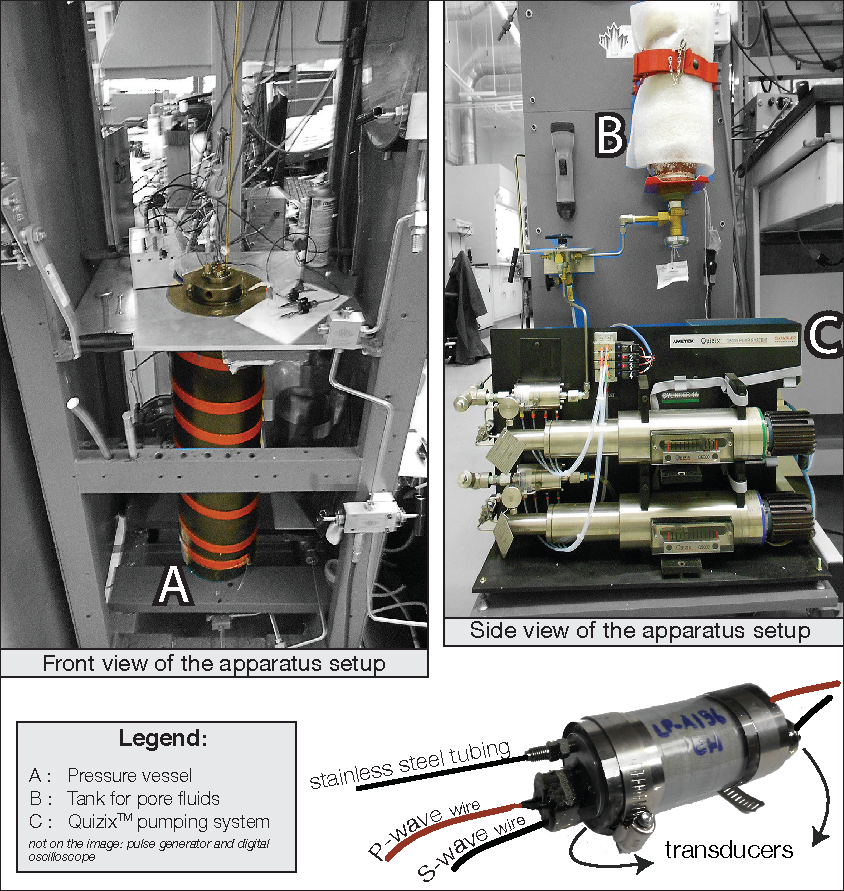
\includegraphics[width=1\textwidth]{fig/apparatus.pdf}
\caption{Apparatus setup and rock sample with transducer assemblage}
\label{fig:apparatus}
\end{figure}
Cylindrical shaped samples of \SI{3.7}{\cm} in diameter having lengths greater
than \SI{4}{\cm}, obtained from CA and CH cores, are used. The ends of the
samples are polished and made as parallel as possible using a surface grinder.
The parallelism is measured using a dial gauge and considered acceptable if it
is within \SI{\pm0.025}{\mm}. Each sample is then dried under vacuum at modest
temperatures (\SI{\sim70}{\degreeCelsius}). It is prepared for the measurement
suite by attaching the set of ultrasonic transducers to its ends. Each
transducer consists of one longitudinal mode and one transverse mode PZT ceramic
glued to an aluminum alloy buffer. The sample-transducers assembly
(\cref{fig:apparatus}) is then hermetically sealed to prevent any contamination
by the hydraulic fluid once the sample is in the pressure vessel. The assembly
is then placed inside the pressure vessel (\cref{fig:apparatus}) in a
cylindrical cavity filled with hydraulic oil. The hydraulic oil serves as the
pressurizing medium for providing hydrostatic confining pressure on the
sample.\\
The \ce{CO2} is introduced into the sample via stainless steel tubing that
connects the pore space of the sample with the pore fluid reservoir located
outside of the vessel. The transmitted seismic signal was generated by
triggering the transducer with a negative spike pulse. For detailed description
of the apparatus see \citet{Njiekak2013} and \citet{Yam2011}.
\subsection{Testing sequence}
The first set of measurements was made with pore space subject to vacuum to
provide the 'dry' properties at different temperature and pressure conditions to
evaluate their effect on the rock frame. The measurements were then repeated
with full \ce{CO2} saturation under a variety of pore pressure at
\SIlist{25;35}{\degreeCelsius} in order to sample the full range of \ce{CO2}
phase states (\cref{fig:bulkdensity}). Finally 'dry' measurements were repeated
to assess any mechanical change that might have altered the rock 'dry'
properties. For each measurements, the sample was left to equilibrate for
\num{5} minutes at constant pressure prior to acquisition of the waveforms. To
reduce random noise effects, the final waveform recorded is a sum of at least
\num{100} traces.
\begin{figure}[!ht]
        \centering
        \begin{subfigure}[b]{.5\textwidth}
                \caption{Density of \ce{CO2}}
                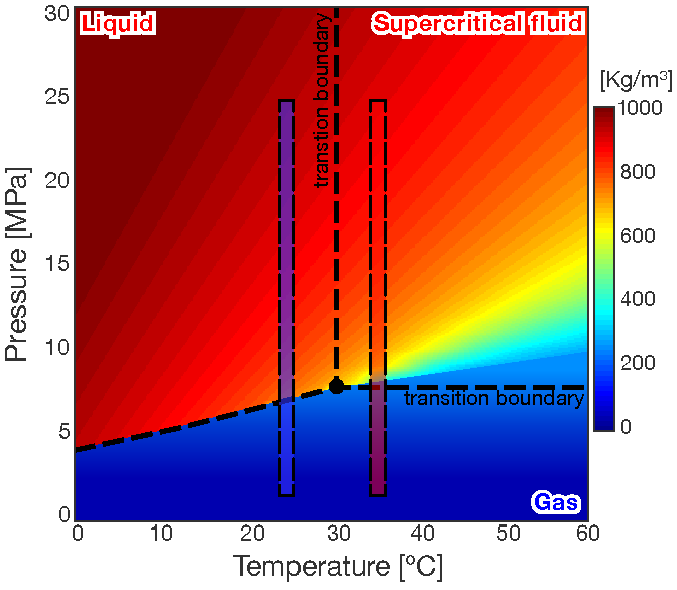
\includegraphics[width=\textwidth]{fig/density.pdf}
                \label{fig:density}
        \end{subfigure}%
        \begin{subfigure}[b]{.5\textwidth}
                \caption{Bulk modulus of \ce{CO2}}
                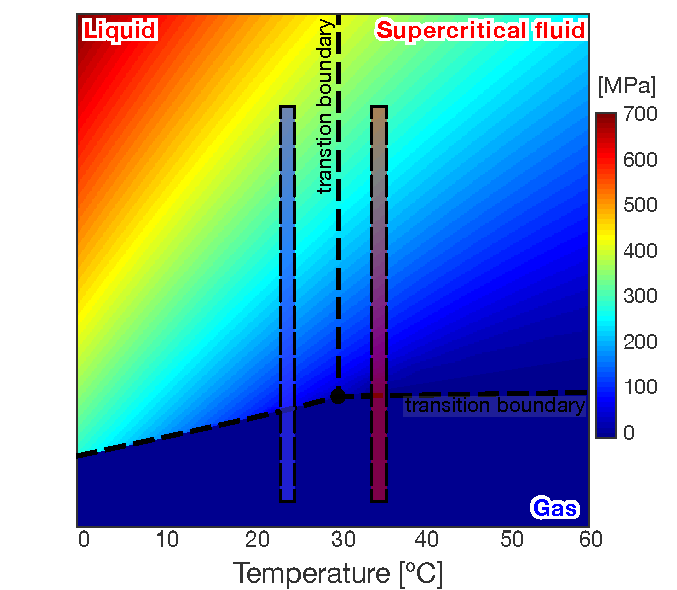
\includegraphics[width=\textwidth]{fig/bulk.pdf}
                \label{fig:bulk}
        \end{subfigure}
        \caption{Phase diagrams of \ce{CO2} based on the thermodynamic model of
\citet{Span1996}. The blue and red bars indicate the P and T conditions for the
experiments runs.}
        \label{fig:bulkdensity}
\end{figure}
\subsection{Experimental results}
An essential characteristic of the measurements was to ensure that the
variations of the waveform are linked only to the change of the properties of
fluids and not to differential pressure dependent changes in the elastic
properties of the rock's frame. Thus, all measurements were carried out at
constant differential pressure of \SI{14}{\mega\pascal} (corresponding to the
expected reservoir conditions) by varying the confining pressure and the pore
pressure according to
\begin{equation}
 P_{d} = P_{c} - P_{p},
\end{equation}
where $P_{d}$ is differential pressure, $P_{c}$ is confining pressure and
$P_{p}$ is pore pressure. As the sample is buffered by two aluminum caps, the
measured travel time must be corrected to obtain the wave velocity $\nu$ of the
sample using
\begin{equation}
 \nu = \frac{L_{s}}{t_{bs}-t_{b}},
\end{equation}
where $L_s$ is the sample length and $t_{bs} - t_{b}$ is the difference between
the travel time through the aluminum buffers and the sample $t_{bs}$, and the
traveltime through the aluminum buffer without the sample $t_b$. The buffer
transit time $t_b$ was determined before the tests that included the samples
over the range of confining pressures and temperatures expected; and this
pressure and temperature dependent values were used in correcting the observed
times through the samples.\\
We present here the measurements made for full \ce{CO2} saturation at two
constant temperature (\SIlist{25;35}{\degreeCelsius}) with the pore pressure
varying from \SIrange[range-units = single]{2}{25}{\mega\pascal} in each case.
Carbon dioxide is in a gaseous state at the lower pores pressures, and in liquid
or supercritical state at higher pore pressures, depending on the temperature as
shown in \cref{fig:bulkdensity}. The suite of $P$-waveforms for CH sample at
\SI{25}{\degreeCelsius} are shown in \cref{fig:waveform_a}.
\Cref{fig:waveform_b} shows how the signal amplitude is picked.  Wave velocities
and relative signal amplitude for $P$- and $S$-wave for the two constant
temperature runs are plotted in \cref{fig:results_lab}. In each subplot curves
for both Cairnside (red) and Covey Hill samples (yellow) are shown.
\begin{figure}[!hb]
        \centering
        \begin{subfigure}[b]{.5\textwidth}
                \caption{normalized P-waveforms over a confining pressure
varying from \SIrange[range-units = single]{2}{25}{\mega\pascal}, red line shows
the first arrival picking.}
                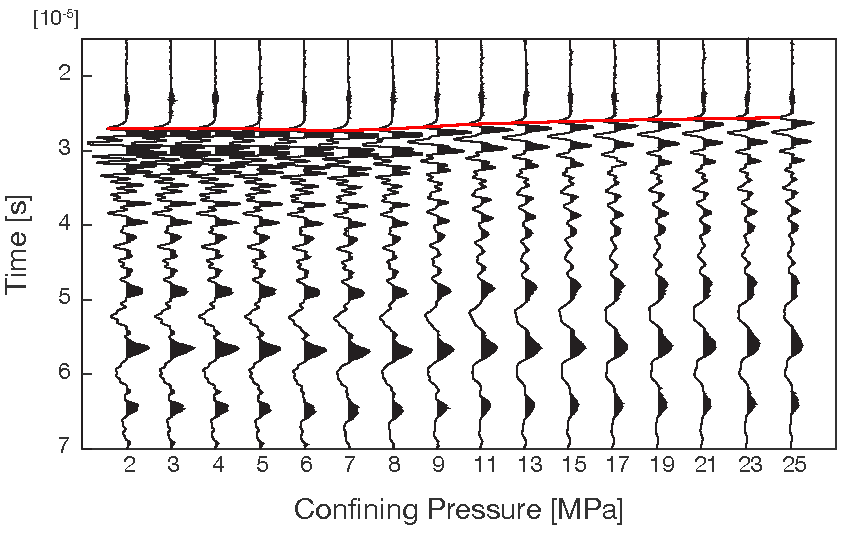
\includegraphics[width=\textwidth]{fig/waveform_a.pdf}
                \label{fig:waveform_a}
        \end{subfigure}%

        \begin{subfigure}[b]{.5\textwidth}
                \caption{Amplitude difference between $P$-waveforms at
\SIlist{2;25}{\mega\pascal}.}
                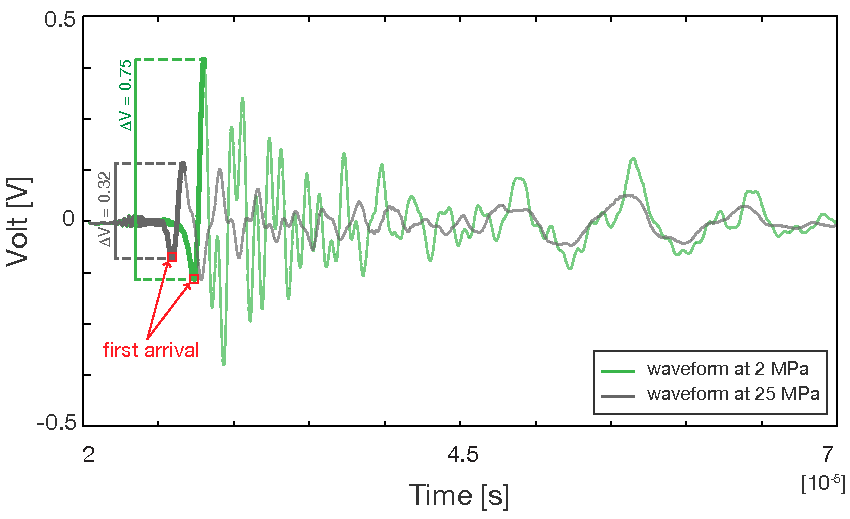
\includegraphics[width=\textwidth]{fig/waveform_b.pdf}
                \label{fig:waveform_b}
        \end{subfigure}

        \caption{P-waveforms of measurements at \SI{35}{\degreeCelsius} for the
CH sample.}
\end{figure}
\subsubsection{Velocity}
For fluid substitution with no change in matrix properties, a change in $P$-wave
velocity is expected due to the change in the saturated bulk modulus
(incompressibility), with a minimal change in $S$-wave velocity expected due to
the lack of change in shear modulus, which is a property presumed to be not
affected by pore fluid \citep{Daley2007}. The change in the bulk density of the
material due to varying \ce{CO2} fluid density is also a significant factor
affecting the wave speeds through the rock. The experimental observations are
summarized as:
\begin{enumerate}[-]
\item $P$-wave velocities (\cref{fig:results_lab_a}) initially decrease with
increasing pore pressure over the range \SIrange{2}{7}{\mega\pascal} for all
runs and for the two samples. These velocities drops are consistent with the
increase of the \ce{CO2} gas density (\cref{fig:density}) as has been observed
in \citep{Yam2011} and \citep{Chowdhury2014}.
\item Once the phase transition is crossed, velocities increase with pore
pressure for both runs. This trend is far more pronounced for the CH sample than
for the CA sample.
\item The pore fluids transition from gaseous \ce{CO2} to liquid/supercritical
\ce{CO2} only concerns $P$-wave velocity. This is confirmed by the lack of sharp
changes in the $S$-wave velocity.
\end{enumerate}
Unfortunately, brine-saturated measurements have not been done due to the salts
dissolved in water which could have damaged the pumping system. However, smooth
velocity variation under water-saturated measurements is expected since water
will not undergo any phase transition based on the applied conditions as
observed by \citet{Njiekak2013}, \citet{Yam2011} and \citet{Chowdhury2014}.
\subsubsection{Signal amplitude}
Signal amplitude (\cref{fig:results_lab_b} and \cref{fig:results_lab_d}) shows a
rapid decrease in the pressure range \SIrange[range-units =
single]{5}{7}{\mega\pascal}. Once the \ce{CO2} phase transition is crossed the
decrease is smoother. This trend is valid for CH sample for both $P$- and
$S$-wave signal, however, for the CA sample, the amplitude decreases steadily
and the phase transition is not clearly detected.\\
Despite the relatively low permeability of the samples, there are substantial
variations on velocity and signal amplitude measurements. Nevertheless, the CH
sample shows a larger sensitivity to \ce{CO2} phase change when compared to the
CA sample. This is attributed to the larger porosity and permeability of the
former (\cref{tbl:prop}).
In the next section, we explore how the higher sensitivity of the CH unit
affects the time-lapse seismic response for a VSP monitoring program.
\begin{landscape}
    \begin{figure*}[p]
        \centering
        \begin{subfigure}[b]{0.563\textwidth}
            \centering
            \caption{$P$-wave velocity}
            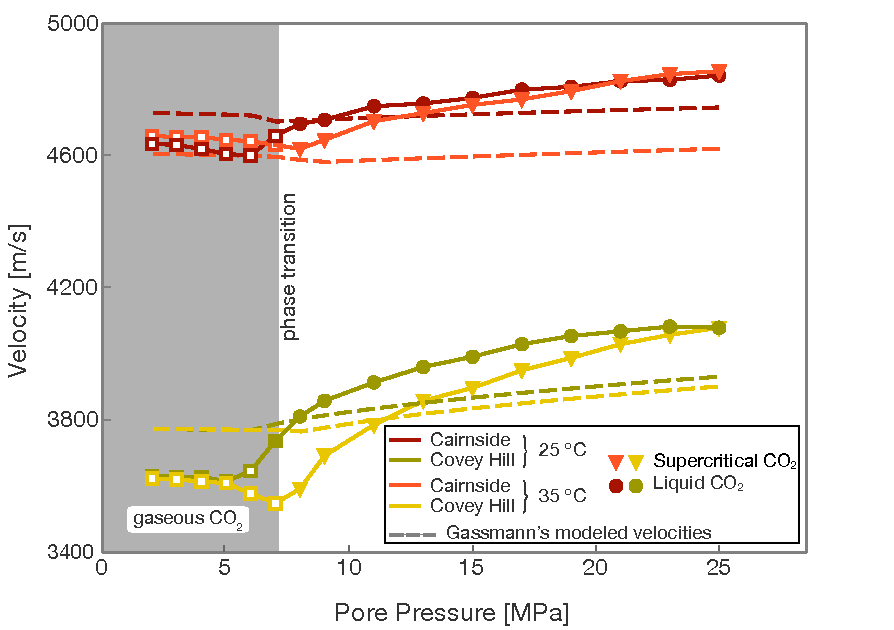
\includegraphics[width=\textwidth]{fig/results_lab_a.pdf}
            \label{fig:results_lab_a}
        \end{subfigure}
        \qquad
        \begin{subfigure}[b]{0.563\textwidth}
            \centering
            \caption{$S$-wave velocity}
            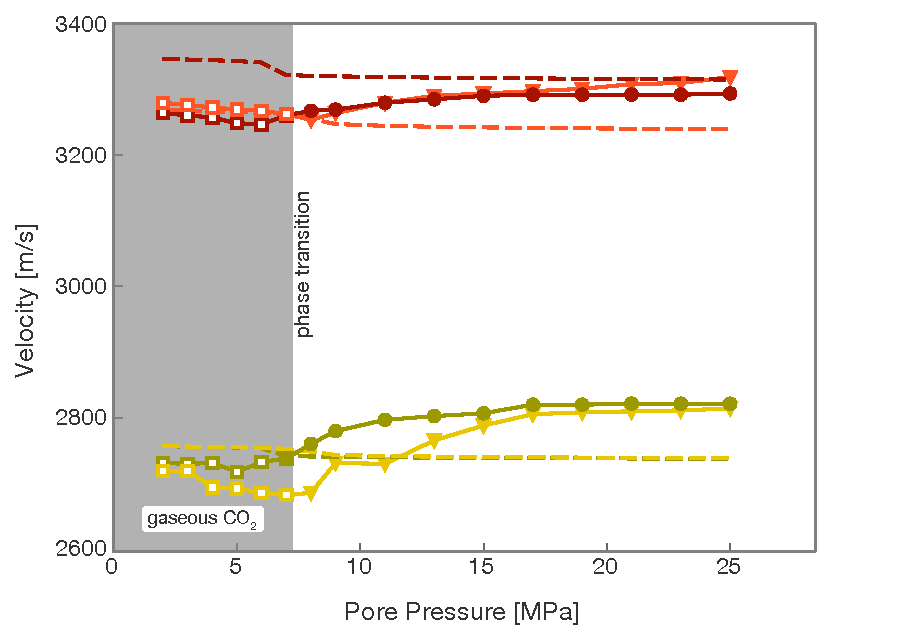
\includegraphics[width=\textwidth]{fig/results_lab_c.pdf}
            \label{fig:results_lab_c}
        \end{subfigure}
        \vskip\baselineskip
        \begin{subfigure}[b]{0.563\textwidth}
            \centering
            \caption{$S$-wave amplitude}
            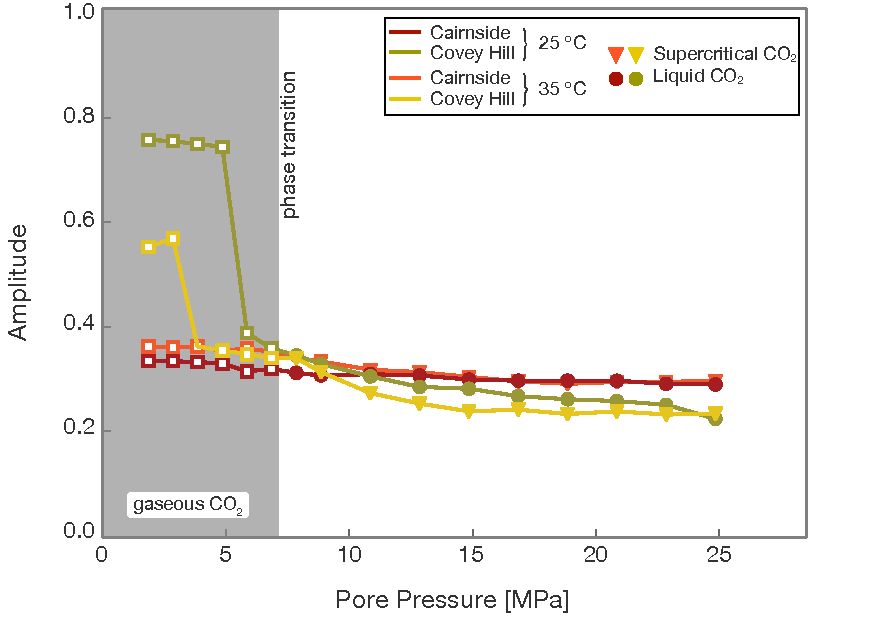
\includegraphics[width=\textwidth]{fig/results_lab_b.pdf}
            \label{fig:results_lab_b}
        \end{subfigure}
        \qquad
        \begin{subfigure}[b]{0.563\textwidth}
            \centering
            \caption{$S$-wave amplitude}
            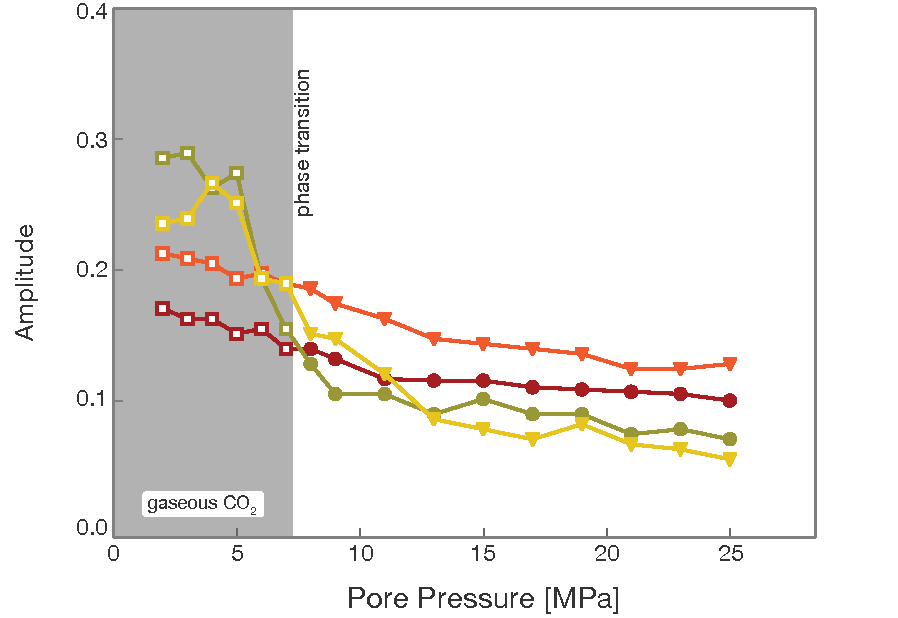
\includegraphics[width=\textwidth]{fig/results_lab_d.pdf}
            \label{fig:results_lab_d}
        \end{subfigure}
        \caption{Velocity and amplitude response for CO$_2$ injection in the
Covey Hill (yellow) and Cairnside (red) samples.}
        \label{fig:results_lab}
    \end{figure*}
\end{landscape}
\subsection{Gassmann modeling}
Applying the laboratory results to seismic monitoring will require the high
frequency data to be scaled down to low frequencies by adequate rock physics
models. Gassmann's relation is largely used to predict the bulk modulus of a
fully saturated rock ($K_{sat}$).  It is a function of the bulk modulus of the
dry rock ($K_{dry}$), the modulus of the fluid ($K_f$), the modulus of the
mineral assemblage ($K_s$), and the rock porosity ($\phi$) \cite{Gassmann}:
\begin{equation}
\label{eq:Kdry}
K_{sat} = K_{dry} +
\dfrac{\bigg(1-\dfrac{K_{dry}}{K_s}\bigg)^2}{\dfrac{\phi}{K_{fl}}+\dfrac{(1-\phi)}{K_s}-\dfrac{K_{dry}}{K^2_s}}.
\end{equation}
Application of Gassmann's equation is based on the assumption that the pore
space is completely connected and the porous frame consists of a single solid
material. Values of the bulk modulus of the minerals composing the studied
sandstones samples are known and not highly variable.  Thus, the effective
mineral bulk modulus $K_s$ can be assumed to be monomineralic with its
properties derived from appropriate averages.\\
Here, $K_s$ is estimated by applying the arithmetic average of the upper and
lower Hashin-Shtrikman bounds \citep{Hashin1963}. For a rock made up of
different minerals, these bounds are formulated as \citep{Barryman1995}:
\begin{equation}
\label{eq:Ks}
K^{HS\pm} = \Lambda(G_{\pm}),
\end{equation}
\begin{equation}
\label{eq:Gs}
G^{HS\pm} = \Gamma \big[\xi(K_{\pm},G_{\pm})\big],
\end{equation}
where
\begin{equation}
\Lambda(G_{\pm}) = \Bigg\langle \dfrac{1}{K_i + \dfrac{4}{3} G_{\pm}}
\Bigg\rangle^{-1}-\dfrac{4}{3}G_{\pm},
\end{equation}
\begin{equation}
\Gamma (\xi) = \bigg\langle\dfrac{1}{G_i + \xi} \bigg\rangle^{-1}-\xi,
\end{equation}
\begin{equation}
\xi(K_{\pm},G_{\pm}) = \dfrac{G_{\pm}}{6}
\bigg(\dfrac{9K_{\pm}+8g_{\pm}}{K_{\pm}+2G_{\pm}}\bigg)
\end{equation}
the subscript $\pm$ denote the maximum and the minimum of the grain constituents
and $K_i$ and $G_i$ are bulk and shear moduli of the $i^{th}$ grain constituent
obtained from \cite{Mavko2009}. The brackets $\langle \cdot \rangle$ indicate an
average over the grain constituents weighted by their volume fractions. The
pressure and temperature dependent bulk modulus ($K_f$) and density ($\rho_f$)
of the \ce{CO2} were determined from the thermodynamic properties obtained from
NIST’s online chemistry webBook \citep{Lemmon2014} and shown in
\cref{fig:bulkdensity}. The $P$- and $S$- wave velocities are then calculated
using \citep{Geertsma1961}:
\begin{equation}
\label{eq:Vp}
V_p = \sqrt{\dfrac{K_{sat}+\dfrac{4}{3}G_{sat}}{\rho_{sat}}},
\end{equation}
and
\begin{equation}
\label{eq:Vs}
V_s = \sqrt{\dfrac{G_{sat}}{\rho_{sat}}}.
\end{equation}
Note that the shear modulus of the saturated rock ($G_{sat}$) is also the shear
modulus of the frame ($G_{dry}$). The saturated bulk modulus is determined from
Gassmann's relation (\cref{eq:Kdry}). The saturated bulk density ($\rho_{sat}$)
is given by
\begin{equation}
\label{eq:rhosat}
\rho_{sat} = (1-\phi)\rho_s + \phi \rho_f.
\end{equation}
Porosity ($\phi$) and grain density ($\rho_s$) of the samples are determined by
means of Hg injection porosimetry.\\
\Cref{fig:results_lab_a} and \cref{fig:results_lab_c} show the modeled
Gassmann's velocities for $P$- and $S$- waves as dashed lines. There is a
general agreement between modeled and measured velocities, though Gassmann's
model over-predicts the measured velocities when the pore fluid is gaseous
\ce{CO2}, except for the CS sample at \SI{35}{\degreeCelsius} and under-predicts
the observed velocities when pore fluid is liquid or supercritical \ce{CO2}.\\
The model assumes that the pores are connected. The rock samples used for the
ultrasonic measurements have a small pore size (\cref{fig:poresize}), which
might restrict the formation of a connective network.
Gassmann's model also assumes that the pressure at the level of the pores is in
equilibrium. It is possible that during the measurements, the pore pressures and
temperatures within the samples did not have sufficient time to stabilize. The
discontinuous changes in wave speed on \cref{fig:results_lab} do not coincide
with the phase boundary. This could be due to the fact that the samples may not
have had sufficient time to change temperature across the phase boundary due to
enthalpy of the phase transition \citep{Kofman2013}. These factors may have
limited the accuracy of the Gassmann's modeling.
\begin{figure}[!ht]
\centering
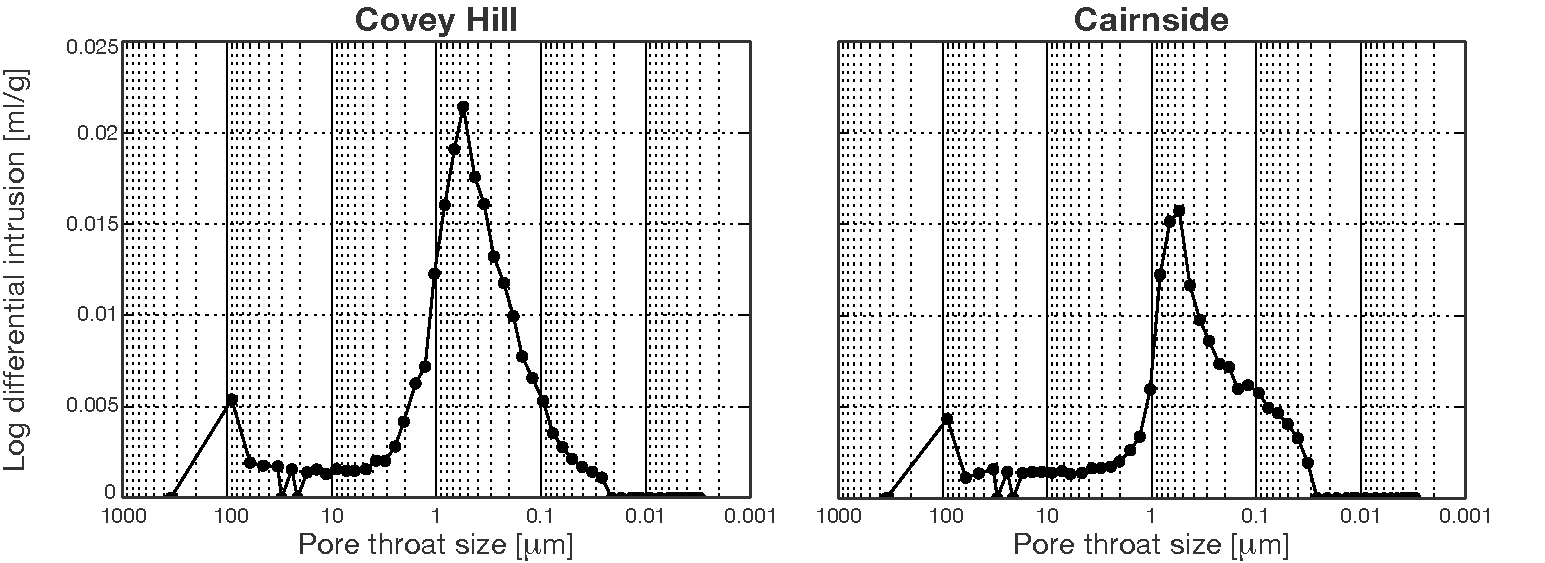
\includegraphics[width=1\textwidth]{fig/pore_size.pdf}
\caption{Log differential intrusion vs. pore size for the matrix of the Covey
Hill and Cairnside samples. Dominant pore throat sizes is
\SI{0.45}{\micro\metre} for both samples.}
\label{fig:poresize}
\end{figure}
\section{Time-lapse seismic response modeling}
Vertical seismic profile (VSP) methods are well suited for pilot carbon
sequestration projects as, on one hand, they provide higher vertical resolution
information than surface seismic \citep{Yang2014} while on the other they allow
for multiple economical repeat surveys. Indeed, VSP surveys for \ce{CO2}
monitoring have been used at pilot-scale \ce{CO2} injection sites such as Ketzin
\citep{Yang2010, Ivandic2012, Gotz2014, Diersch2014}, SACROC
\citep{Yang2014,Cheng2010}, Frio \citep{Daley2007}, and Otway
\citep{Urosevic2008}. VSP methods have been also used in commercial projects
such as IEA GHG Weyburn-Midale \ce{CO2} Monitoring and Storage Project
\citep{Bellefleur2004} and Aquistore \citep{White2014}.\\
 For this study, numerical simulation of time-laspe VSP surveys has been
conducted as preparatory work for a future VSP monitoring program.
\subsection{Methodology}
Seismic modeling is a technique for simulating wave propagation in the earth.
The objective is to predict a seismogram given a composition and structure of
the subsurface \citep{Carcione2010}. Seismic wave propagation can be modeled by
solving the wave equations for acoustic, elastic, viscoelastic, poroelastic or
poro-viscoelastic media. The procedure followed in this study to perform seismic
modeling is directly inspired by the work of \citet{Carcione2006} who present an
application of poro-viscoelastic modeling for monitoring underground \ce{CO2}
storage. The poro-viscoelastic formulation represents perhaps the most effective
tool to study the effect of the saturating fluid on the seismic response because
fluid properties are directly taken into account in the equations. It is thus
not necessary to rely on fluid substitution models to compute effective seismic
moduli, and it is expected that fluid substitution effects are mode accurately
described. The modeling code used in this work is described in
\citet{Giroux2012}.\\
The elastic coefficients characterizing the porous media introduced by
\citet{Biot1957} and reported in \citet{Carcione1998} are:\\
The $P$-wave modulus of the matrix ($E$)
\begin{equation}
E = K_{dry} + \dfrac{4}{3}G,
\end{equation}
The coupling modulus ($M$) between the solid and the fluid
\begin{equation}
M = \dfrac{K_{s}^{2}}{D-K_{dry}} ,
\end{equation}
where the diffusion fucntion D is defined as
\begin{equation}
D = K_s \big[1 + \phi(K_s K_{f}^{-1} -1)\big],
\end{equation}
The poroelastic coefficient ($\alpha$) of effective stress
\begin{equation}
 \alpha = 1 - \dfrac{K_{dry}}{K_s},
\end{equation}
where $K_{dry}$, $K_s$, $K_f$ are the bulk moduli of the drained matrix, the
solid and the fluid respectively; $\phi$ is the porosity, and $G$ is the shear
modulus of the matrix (both cases of drained and saturated).
 \citet{Carcione1998} presented an approach to introduce viscoelasticity into
Biot's poroelastic equations, in which matrix-fluid mechanisms are modeled by
generalizing the coupling modulus $M$ to a time dependent relaxation function
while the others elastic coefficients are independent of frequency. Detailed
information on the implementation of the equations of motion can be found in
\citet{Carcione1998} and \citet{Carcione1999}.
\subsection{Geological model}
We consider a 2D idealized geometry and physical model to describe the
sedimentary sequence of the St. Lawrence Lowlands. The geological model consists
of a tabular succession of six horizontal layers corresponding to the Lorraine
group, Utica shales, Trenton group, Beekmantown group, Cairnside formation,
Covey Hill formation and the Grenville basement. The grid size is \SI{2000 x
1500}{\metre} with a cell size is \SI{1 x 1}{\metre}, leading to a total of
\num{3} million cells. For each cell, \num{11} parameters
($K_{dry},K_s,K_f,\phi,G_s,\rho_s,\rho_f,\tau,\eta,\kappa,Q$ -
\Cref{tbl:modelpar}) characterize the medium.
A sequential Gaussian simulation (SGS) framework is used to modify the classical
geological blocky model in order to obtain a more realistic heterogeneous model.
First, for each layer, we compute the mean ($\mu$) and the standard deviation
($\sigma$) of the physical properties (mineralogical composition (V$_{clay}$,
V$_{calcite}$, V$_{quartz}$, V$_{dolomite}$), $V_p$, $V_s$, porosity($\phi$) and
density ($\rho$) derived from log data available in the studied region. The dry
laboratory measurements are used to obtain the dry-rock bulk modulus that is one
main component of the model. The distribution of the physical properties are
then obtained by simple kriging under Gaussian hypothesis and used for computing
the model parameters as the following:\\
the dry-rock bulk modulus ($K_{dry}$) is estimated using inverse Gassmann's
equation \citep{Hamilton1971,Carcione2007}:
\begin{equation}
K_{dry} = \dfrac{(\phi \dfrac{K_s}{K_f} + 1 - \phi)K_{sat} - K_s}{\phi
\dfrac{K_s}{K_f} + \dfrac{K_{sat}}{K_s} - 1 - \phi},
\end{equation}
where $K_{sat} = \rho V_{P}^{2} - (4/3)G$ is the saturated bulk modulus.\par
The bulk ($K_s$) and shear ($G_s$) moduli of the solid are estimated using
\cref{eq:Ks} and (\ref{eq:Gs}) - see \cref{tbl:mineralpost} for the mineralogic
composition.
Tortuosity ($\tau$) is estimated using \citep{Glover2009}:
\begin{equation}
\tau = \phi^{1-m},
\end{equation}
where $m$ is the cementation factor.
The brine properties are obtained by using the equations given in
\citet{Batzle1992}. The pressure and temperature dependent bulk modulus ($K_f$),
density ($\rho_f$) and viscosity ($\eta_f$) of the \ce{CO2} are determined from
the thermodynamic properties obtained from NIST’s online chemistry webBook
\citep{Lemmon2014}. Permeabilities ($\kappa$) are taken from
\citet{TranNgoc2014}. The velocity fields for the heterogeneous and for the
classical block models are shown in \cref{fig:mstochvsblock}.
\begin{table}[!h]
%\ra{1}
  \centering
  \caption{Mineral composition of the Potsdam group sandstones.}
\begin{tabular}{lS[table-number-alignment = center,table-format =
2.0]S[table-number-alignment = center,table-format = 2.0]}
\toprule
 & {Cairnside} & {Covey Hill}\\
  & {\small{(\si{\percent})}} & {\small{(\si{\percent})}}\\
\midrule
 Quartz   & 90 & 82 \\
 Smectite  & 6 & 12 \\
 Calcite  & 2 & 3 \\
Dolomite  & 2 & 2 \\
\bottomrule
\end{tabular}
\label{tbl:mineralpost}
\end{table}
% \afterpage{
\begin{landscape}
\begin{table}[p]
  \caption{Parameters defining the geological model}
  \label{tbl:modelpar}
  \sisetup{}
  \centering
	\begin{threeparttable}[b]
	\begin{tabular}{@{}l
	S[table-format = 2.2]
	S[table-format = 3.2]
	S[table-format = 1.3]
	S[table-format = 2.2]
	S[table-format = 2.2]
	S[table-format = 4.0]
	S[table-format = 4.0]
	S[table-format = 2.2]
	S[table-format = 1.2]
	S[table-format = 1.1e-2]
	S[table-format = 3.2]
	@{}}
\toprule

& \textbf{$K_{dry}\tnote{*}$} & \textbf{$K_s$}\tnote{*} & \textbf{$K_f$} &
\textbf{$\phi$}\tnote{*} & \textbf{$G_s$}\tnote{*} & \textbf{$\rho_s$}\tnote{*}
& \textbf{$\rho_f$} & \textbf{$\tau$}\tnote{*} & \textbf{$\eta$} &
\textbf{$\kappa$} & \textbf{$Q$}\tnote{*} \\
& \scriptsize{dry rock} & \scriptsize{bulk modulus} & \scriptsize{bulk modulus}
& \scriptsize{porosity} & \scriptsize{shear} &\scriptsize{density }
&\scriptsize{density } & \scriptsize{tortuosity}&\scriptsize{fluids }
&\scriptsize{permeability} &\scriptsize{seismic } \\
& \scriptsize{bulk modulus} & \scriptsize{of the grains} & \scriptsize{of the
fluids}  &  & \scriptsize{modulus} &\scriptsize{of the grains} &\scriptsize{of
the fluids} & & \scriptsize{viscosity}& &\scriptsize{quality factor} \\
& \footnotesize{(\si{\giga\pascal})} & \footnotesize{(\si{\giga\pascal})} &
\footnotesize{(\si{\giga\pascal})}  &  \footnotesize{(\si{\percent})}
&\footnotesize{(\si{\giga\pascal})} &\footnotesize{(\si{\kg\per\cubic\metre})} &
\footnotesize{(\si{\kg\per\cubic\metre})}& \footnotesize{(-)}&
\footnotesize{(cP)}& \footnotesize{(\si{\metre\squared})}&\footnotesize{(-)} \\
\midrule

\multirow{2}{*}{Lorraine} & 9.91 & 50.62 & 2.3 & 14 & 9.14 & 2621 & 1000 & 2.67
& 1 & 1.9e-19 & 110 \\
						  &  & &&&&&&&&\\
\multirow{2}{*}{Utica shales} & 22.15 & 76.80 & 2.3 & 4.7 & 17.97 & 2662 & 1000
& 5.70 & 1 &  1.9e-19 & 141 \\
							  & &&&&&&&&&\\
\multirow{2}{*}{Trenton} & 34.44 & 108.59 & 3.2 & 1.6 & 23.85 & 2711 & 1150 &
18.96 & 1.3 &  1.9e-16 & 168 \\
						 & &&&&&&&&&\\
\multirow{2}{*}{Beekmantown} & 25.37 & 80.66 & 3.072 & 1.9 & 26.58 & 2704 & 1120
& 18.89 & 1.1 & 1.5e-16 & 156 \\
							 & &&&&&&&&&\\
\multirow{2}{*}{Cairnside} & 18.70 & 62.76 & 3.55 & 3.55 & 19.36 & 2662 & 1190 &
19.65 & 1.28 & 1.2e-16 & 133 \\
						   & &&&&&&&&&\\
\multirow{2}{*}{Covey Hill} & 16.27 & 65.25 & 2.9 & 6.6 & 18.73 & 2664 & 1090 &
12.08 & 1 & 2.4e-16 & 136 \\
							& &&&&&&&&&\\
\multirow{2}{*}{Basement} & 37.82 & 119.28 & 3.4 & 1.6 & 32.25 & 2670 & 1200 & 1
& 1 & 1.0e-19 & 175 \\
						  & &&&&&&&&&\\
\bottomrule
\end{tabular}
\begin{tablenotes}
\item [*] Mean values representing parameters that have been simulated.
\end{tablenotes}
\end{threeparttable}
\end{table}
\end{landscape}
% }
\begin{figure}[!ht]
        \centering
        \begin{subfigure}[b]{1\textwidth}
                \caption{Heterogeneous realistic model.}
                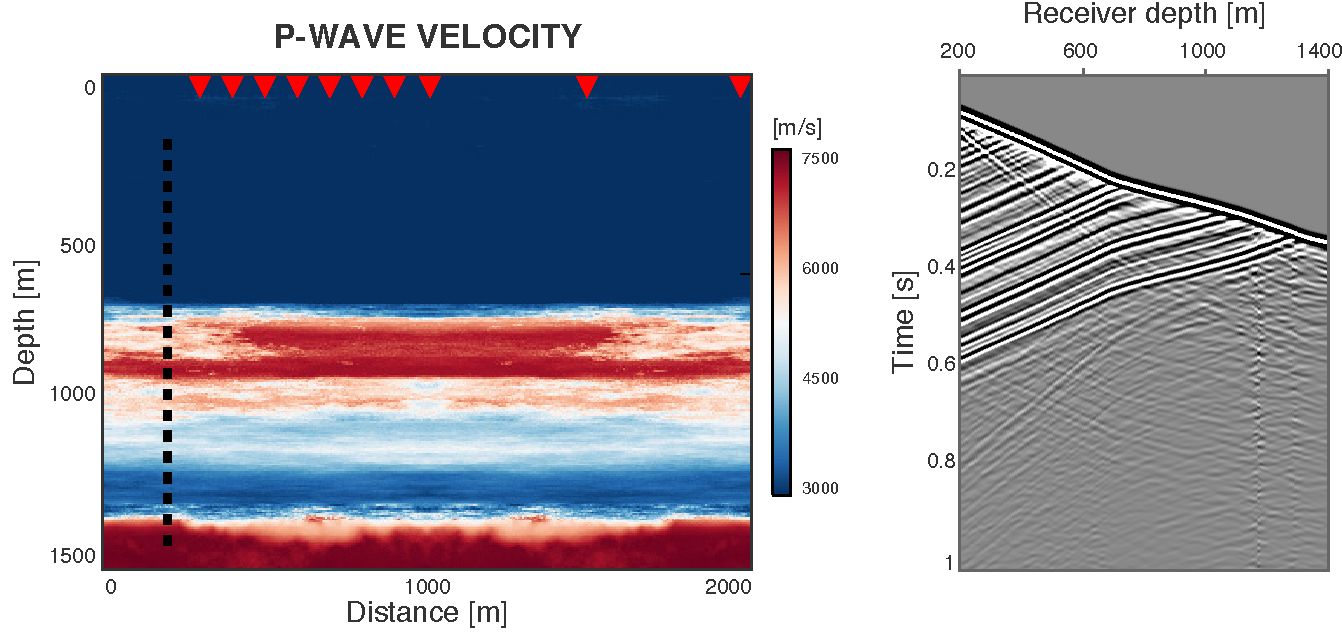
\includegraphics[width=\textwidth]{fig/model_stochvsblock_a.pdf}
                \label{fig:mstochvsblock_a}
        \end{subfigure}%

        \begin{subfigure}[b]{1\textwidth}
                \caption{Classical block model.}
                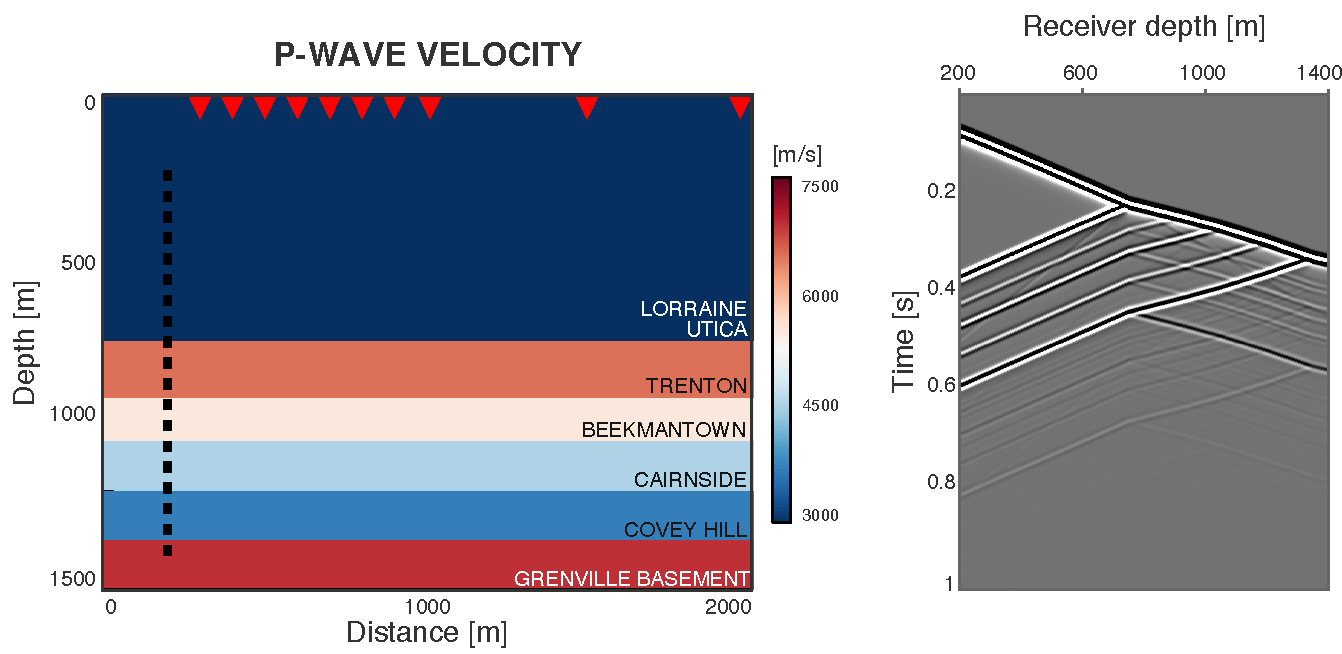
\includegraphics[width=\textwidth]{fig/model_stochvsblock_b.pdf}
                \label{fig:mstochvsblock_b}
        \end{subfigure}

        \caption{$P$-wave velocity for the heterogeneous and block model with
respectively seismograms.}
        \label{fig:mstochvsblock}
\end{figure}
\subsection{\texorpdfstring{\ce{CO2}}{CO2} injection modeling}
Modeling the seismic response to \ce{CO2} injection requires representative
models to correctly predict the system behavior. This implies fluid flow
modeling to predict the progression of \ce{CO2} plume in the reservoir. The
classic approach relies on three-dimensional numerical methods to solve the
system with a high degree of accuracy. However, this involves significant
computational efforts that are not always feasible. In recent years, approaches
that employ semi-analytical methods have been increasingly developed
\citep{Nordbotten2005a, Nordbotten2009}. One promising simulation tool for fast
and accurate modeling of \ce{CO2} sequestration is based on the vertical
equilibrium (VE) assumption. VE models have a long tradition for describing
flows in porous media; in hydrology it is known as the Dupuit approximation,
whereas in the oil industry is used to simulate two-phase and three phase
segregated flow \citep{Martin1958,Coats1967,Martin1968}. In recent years, VE
methods have been employed to simulate large scale \ce{CO2} injection and
migration, for which a sharp interface assumption with vertical equilibrium may
be reasonable due to the large density difference between supercritical \ce{CO2}
and brine \citep{Nordbotten2005a,Celia2006, Nordbotten2006}.\\
For the purpose of this study, we used the VE solvers included in the Matlab
Reservoir Simulation Toolbox (MRST) \citep{Lie2011}, to model the \ce{CO2}
injection, where the heterogeneous geological model built in the previous
section is used as input. Two different scenarios are proposed: an optimistic
scenario (\cref{fig:seismopt}), where  porosity and permeability reflect those
of the Ketzin pilot project \citep{Michael_2010}, and a Bé\-can\-cour-like
scenario (\cref{fig:seismbec}). The model simulates injection of \ce{CO2} in the
Potsdam formations during \num{15} years at an injection rate of
\SI{45}{\tonne\per\day}. This rate is comparable to the average rate for
injection at Ketzin \citep{Martens_2012}. This injected \ce{CO2} allowed to
migrate further outward for the next \num{35} years. The total storage of
\ce{CO2} is \SI{245}{\kilo\tonne}. The properties of the model are summarized in
\cref{tbl:co2par}. The \ce{CO2} plume for the Bé\-can\-cour-like scenario is
limited to a few hundreds of meters around the well due to its low
permeabilities and porosity. The results are consistent with those obtained by
\citet{TranNgoc2013} using TOUGH2 \citep{Pruess1999,Pruess2005}. For the
optimistic scenario (where permeabilities and porosities are respectively
\numlist{2000;2} times greater than the Bé\-can\-cour-like scenario), the plume
extends for more than a kilometer. During the migration time the \ce{CO2} is
partially dissolved for the latter scenario, while it is not the case in the
Bé\-can\-cour-like scenario.
\begin{figure}[!ht]
        \centering
        \begin{subfigure}[b]{0.95\textwidth}
                \caption{5 years monitoring}
                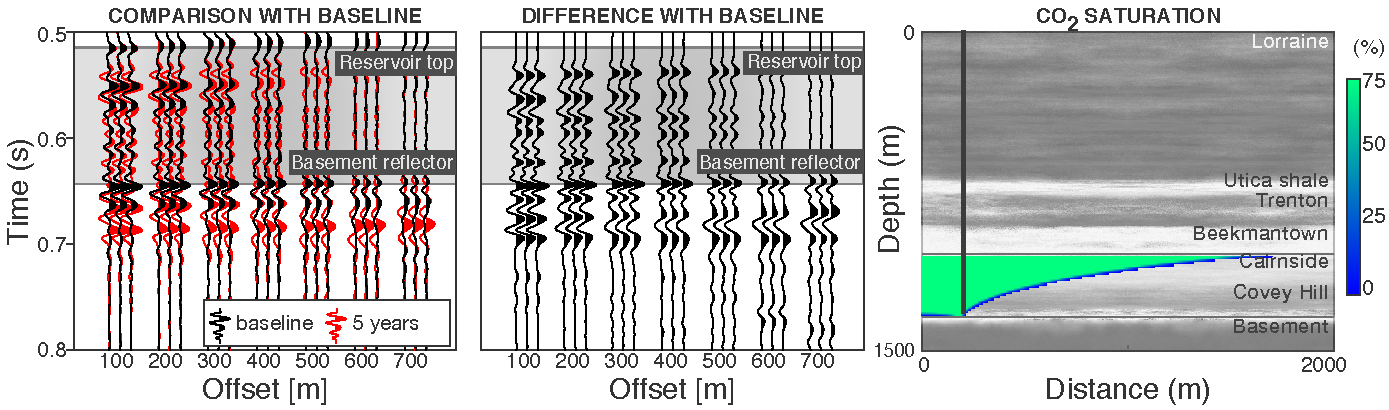
\includegraphics[width=\textwidth]{fig/seism_opt_new_a.pdf}
                \label{fig:seism_opt_a}
        \end{subfigure}%

        \begin{subfigure}[b]{.95\textwidth}
                \caption{15 years monitoring}
                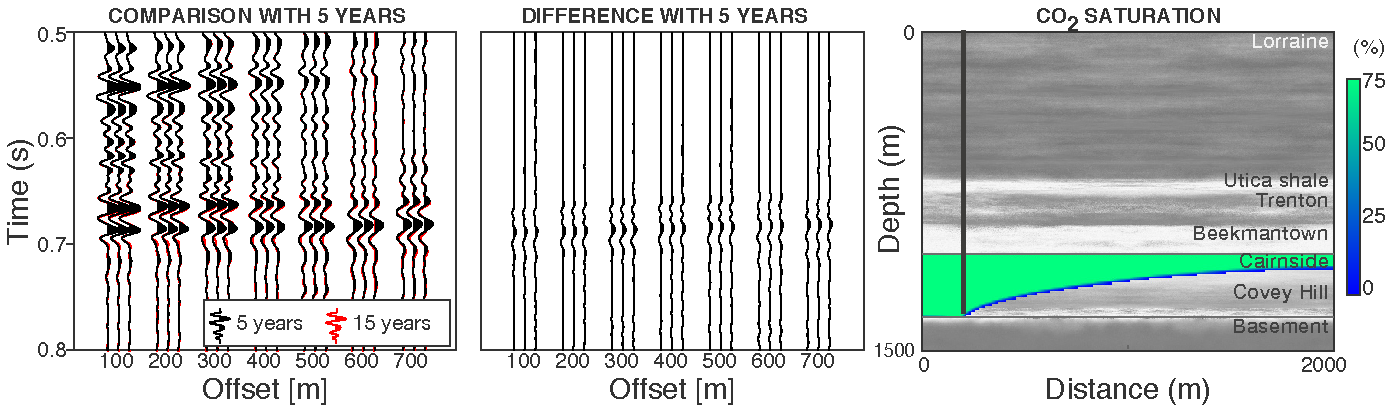
\includegraphics[width=\textwidth]{fig/seism_opt_new_b.pdf}
                \label{fig:seism_opt_b}
        \end{subfigure}

        \begin{subfigure}[b]{.95\textwidth}
                \caption{50 years monitoring}
                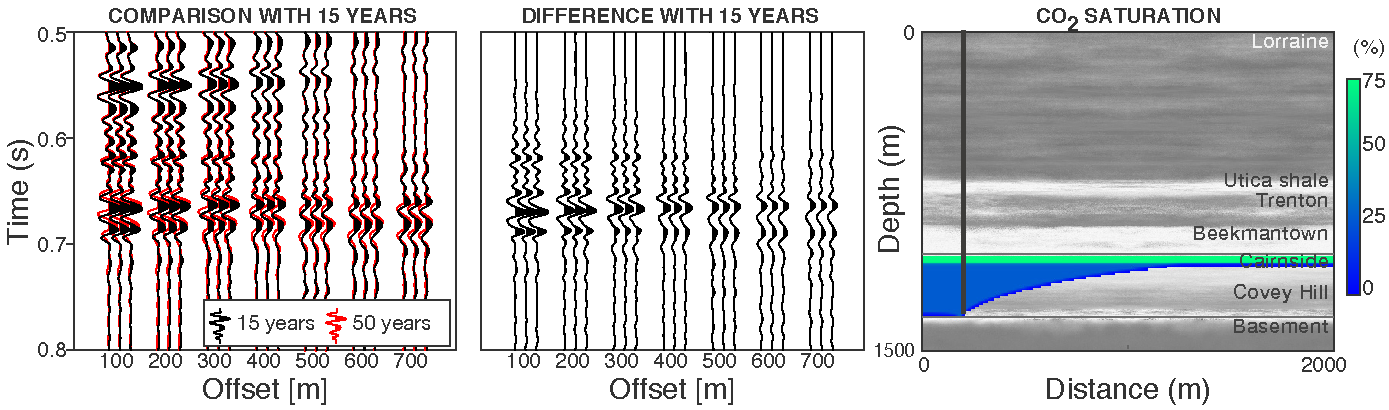
\includegraphics[width=\textwidth]{fig/seism_opt_new_c.pdf}
                \label{fig:seism_opt_c}
        \end{subfigure}

        \caption{Corridor stack difference (3 traces for each offset) for the
optimistic scenario.}
        \label{fig:seismopt}
\end{figure}

\begin{figure}[!ht]
        \centering
        \begin{subfigure}[b]{0.95\textwidth}
                \caption{5 years monitoring}
                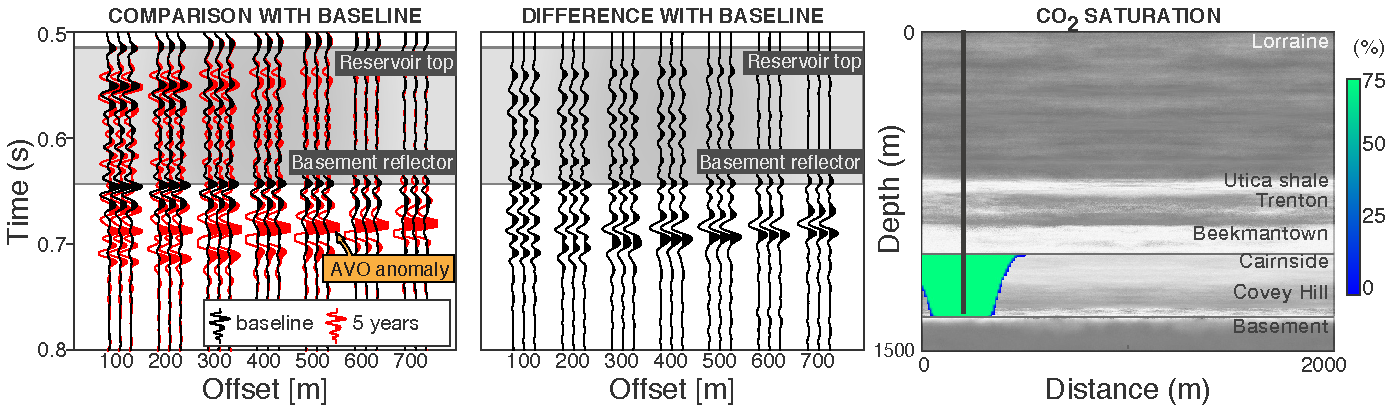
\includegraphics[width=\textwidth]{fig/seism_bec_new_a.pdf}
                \label{fig:seism_bec_a}
        \end{subfigure}%

        \begin{subfigure}[b]{.95\textwidth}
                \caption{15 years monitoring}
                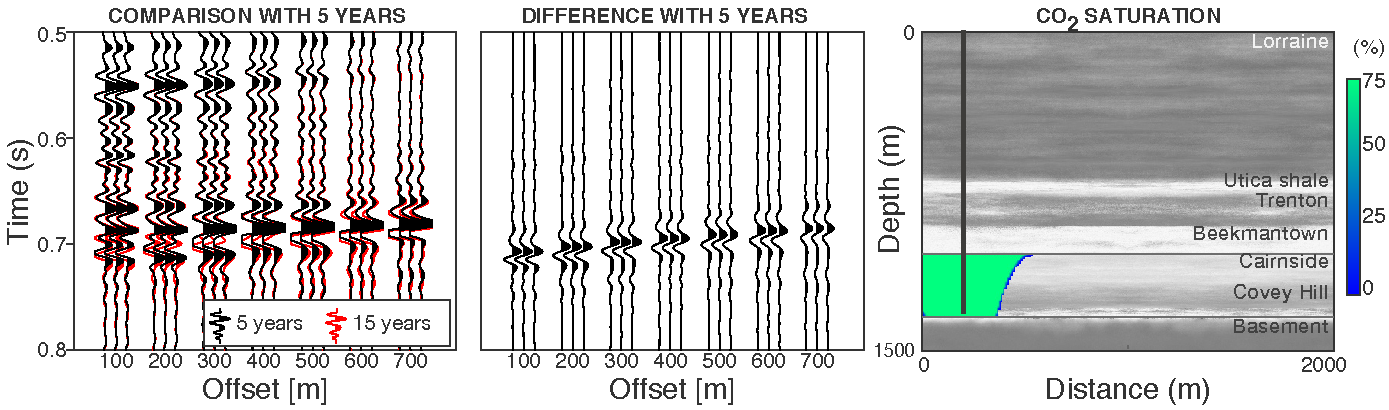
\includegraphics[width=\textwidth]{fig/seism_bec_new_b.pdf}
                \label{fig:seism_bec_b}
        \end{subfigure}

        \begin{subfigure}[b]{.95\textwidth}
                \caption{50 years monitoring}
                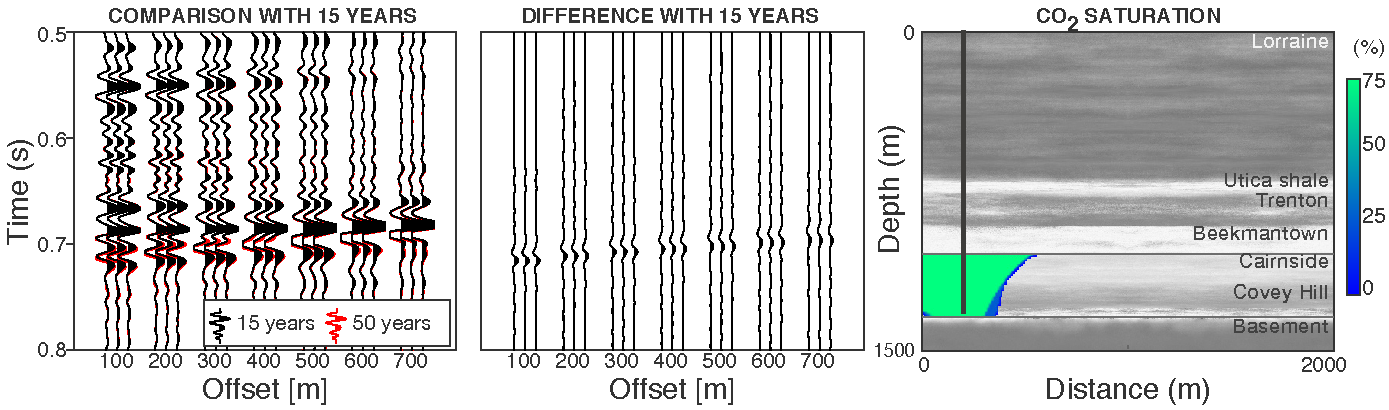
\includegraphics[width=\textwidth]{fig/seism_bec_new_c.pdf}
                \label{fig:seism_bec_c}
        \end{subfigure}

        \caption{Corridor stack difference (3 traces for each offset) for the
B\'e\-can\-cour like scenario.}
        \label{fig:seismbec}
\end{figure}
\begin{table}
  \centering
  \caption{Models parameters for the \ce{CO2} injection simulation and for
synthetics seismograms}
 \begin{tabular}{p{3.5cm}lSS}
\toprule
  && {\textbf{Bé\-can\-cour-like}} & {\textbf{Optimistic}}   \\
\cmidrule(r){3-4}
Avg. porosity at reservoir &(\si{\percent})  &  6  &  20   \\
Avg. permeability & (\si{\metre\squared})  & 3.06e-16  & 6.5e-13  \\
x range &(\si{\metre}) & \multicolumn{2}{c}{2000 }  \\
z range &(\si{\metre}) & \multicolumn{2}{c}{1500 }  \\
Injection depth &(\si{\metre}) & \multicolumn{2}{c}{1200-1350 }  \\
Injection rate &(\si{\tonne\per\metre}) & \multicolumn{2}{c}{45 }  \\
Injection time &(years) & \multicolumn{2}{c}{15 }  \\
Migration time &(years) & \multicolumn{2}{c}{35}  \\
Total storage &(\si{\kilo\tonne}) & \multicolumn{2}{c}{245}\\
Source offsets &(\si{\metre}) & \multicolumn{2}{c}{100, 200, 300, 400, 500, 600,
700}    \\
Receiver x coordinate &(\si{\metre}) & \multicolumn{2}{c}{200} \\
Receiver z coordinate &(\si{\metre}) & \multicolumn{2}{c}{200-1400} \\
Receiver spacing &(\si{\metre}) & \multicolumn{2}{c}{5} \\
Total traces & & \multicolumn{2}{c}{241} \\
\bottomrule
\end{tabular}
\label{tbl:co2par}
\end{table}
\subsection{Synthetic seismograms}
The aim of the modeling exercise is to simulate time-lapse VSP surveys. We are
interested in analyzing what is the effect of the injected \ce{CO2} after
\numlist{5;15;50} years from the start of injection as shown in
\cref{fig:seismopt,,fig:seismbec}. Large (\SI{>700}{\metre}) amplitude versus
offset analysis (AVO) \citep{Backus1982,Ostrander1982,Ostrander1984} in our work
are compromised due to a refracted wave (\cref{fig:refracted}) that arises at
the interface between the Lorraine/Utica shales and Trenton group, preventing a
proper separation of upgoing and downgoing waves. The parameters for the
synthetic seismograms are summarized in \cref{tbl:co2par}.
% \begin{figure}[!ht]
% \centering
% 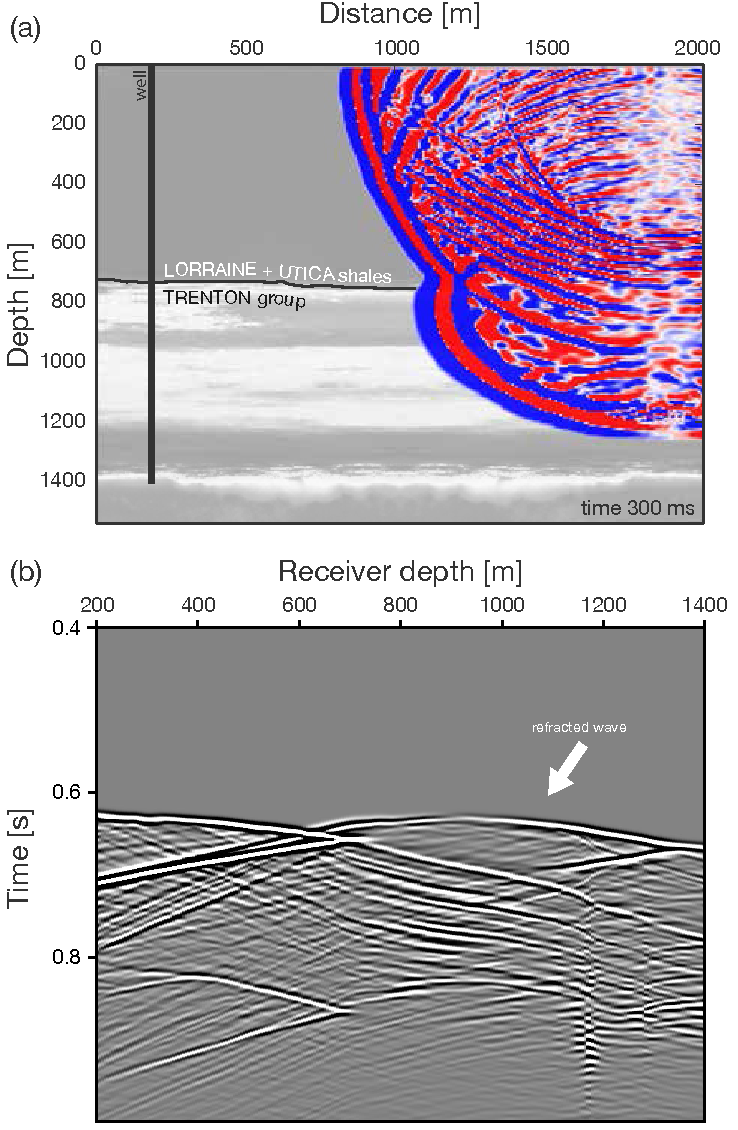
\includegraphics[width=0.8\textwidth]{fig/refracted_new.pdf}
% \caption{Refracted wave that arise at large offset (\SI{>700}{\metre}). a)
% Snapshot of the wave propagation at 300 ms and b) resulting seismogram.}
% \label{fig:refracted}
% \end{figure}
\begin{figure}[!ht]
        \centering
        \begin{subfigure}[b]{0.75\textwidth}
                \caption{Snapshot of the wave propagation at 300 ms for source
placed at \SI{2000}{\metre}.}
                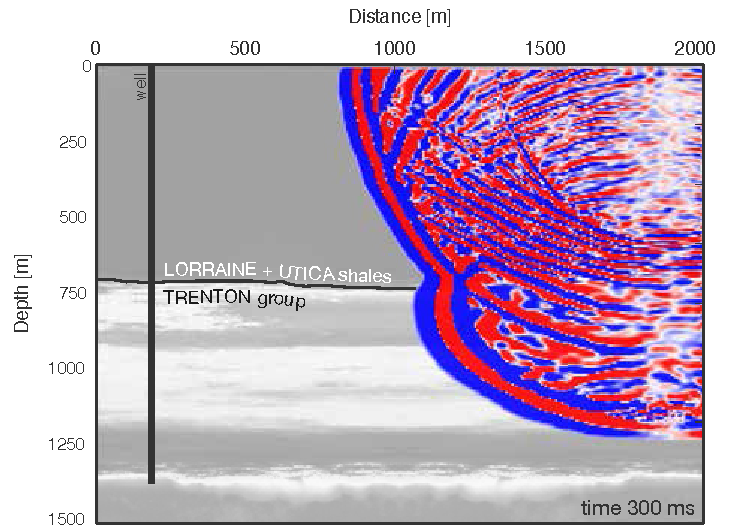
\includegraphics[width=1\textwidth]{fig/refracted_new_a.pdf}
                \label{fig:refracted_a}
        \end{subfigure}%

        \begin{subfigure}[b]{0.75\textwidth}
                \caption{Resulting seismogram.}
                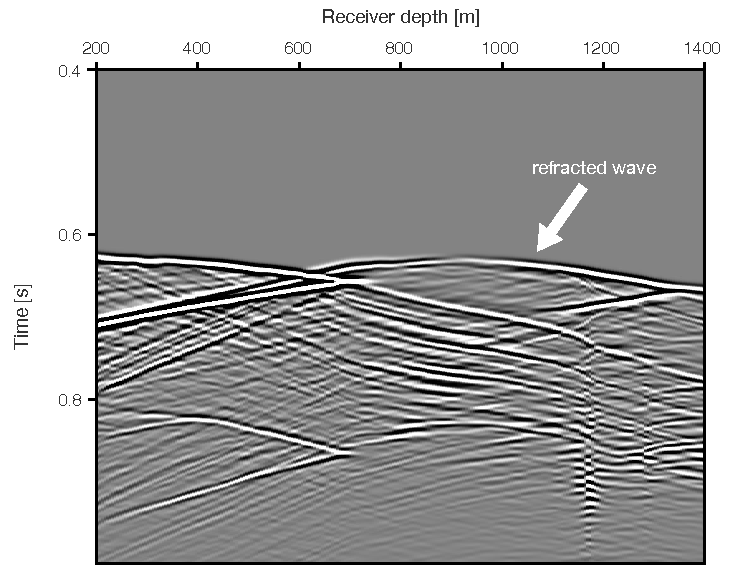
\includegraphics[width=1\textwidth]{fig/refracted_new_b.pdf}
                \label{fig:refracted_b}
        \end{subfigure}

        \caption{Refracted wave that arise at large offset (\SI{>700}{\metre}).}
        \label{fig:refracted}
\end{figure}


\begin{table}
%\ra{1}
  \centering
  \caption{Synthetic seismogram processing}
\begin{tabular}{@{}cl@{}}
\toprule
 \textbf{Step} & \textbf{Processing operation}\\
\midrule
1   & Trace edit \\
2  & Pick first arrival  \\
3 & Velocity analysis on the zero offset shot\\
4  & f-k filter to separate upgoing and downgoing waves \\
5 & NMO analysis\\
6 & Static: flatten the upgoing wave using the first arrivals  \\
7 & VSP corridor mute\\
8 & VSP stack (3 traces)\\
 \bottomrule
\end{tabular}
\label{tbl:process}
\end{table}
\subsection{Modeling results}
In this section we present the results of three synthetic seismograms, for 5, 15
and 50 years after the start of CO$_2$ injection, for both B\'ecancour and
optimistic scenarios (\cref{fig:seismbec,fig:seismopt} respectively).
% \Cref{fig:seism_opt_a,fig:seism_bec_a} show the results for 5 years
% monitoring; \cref{fig:seism_opt_b,fig:seism_bec_b} show the results for 15 year
% monitoring and \cref{fig:seism_opt_c,fig:seism_bec_c} show the results for 50
% year monitoring.
The processing has been inspired by the work of \citet{Coulombe1996,Zhang2010};
the main steps are summarized on \cref{tbl:process}.
\subsubsection{Optimistic scenario}
\Cref{fig:seismopt} shows the corridor stack (\num{7} offsets) for the
optimistic scenario. \Cref{fig:seism_opt_a} shows the comparison and the
difference between baseline and \num{5} years monitoring. The effect of \ce{CO2}
 is mainly observed by a travel-time delay starting at \SI{550}{\ms}. Other
authors reported similar observations \citep{Yang2014,Arts2004}. The delay is
evaluated by crosscorrelation between baseline and 5 years timelapse for each
offset and is of about 30 ms as showed in \cref{tbl:delay}.
\Cref{fig:seism_opt_b} shows the comparison and the difference between
\numlist{5,15} years monitoring. The differences detected are minimal. This is
confirmed by the shape of the \ce{CO2}  plume that after \num{15} years of
injections has the same shape than after \num{5} years. \Cref{fig:seism_opt_c}
shows the comparison and the difference between \numlist{15,50} years
monitoring. The \ce{CO2}  injection modeling show that during migration time
(\numrange{15}{50} years) there is partial dissolution of \ce{CO2} . This is
reflected in the \num{50} years (red traces), with reflections that arrive
\SI{5}{\ms} earlier when compared to the \num{15} years (black traces).
\begin{table}[!bh]
%\ra{1}
  \centering
  \caption{Signal delay between the baseline survey and seismic traces collected
5 years after the CO2 injection.}
\begin{tabular}{@{}cc@{}}
\toprule
  Offset (m) & Delay (ms)\\
  % & \small{[\%]} & \small{[\%]}\\
\midrule
 100   & 22.50  \\
 200   & 23.00  \\
 300   & 33.75  \\
 400   & 33.00  \\
 500   & 31.50  \\
 600   & 30.75  \\
 700   & 30.25  \\
 \textbf{mean}  & \textbf{29.25}  \\
\bottomrule
\end{tabular}
\label{tbl:delay}
\end{table}
\subsubsection{Bécancour scenario}
\Cref{fig:seismbec} shows the corridor stack (7 offsets) for the Bécancour
scenario. \Cref{fig:seism_bec_a} shows the comparison and the difference between
baseline and \num{5} years monitoring. As for the optimistic scenario, the
effect of \ce{CO2} is mainly observed by a travel-time delay starting at
\SI{550}{\ms}. \Cref{fig:seism_bec_b} shows the comparison and the difference
between \numlist{5,15} years monitoring. The differences are highlighted at
\SI{700}{\ms} due to the greater extension of the \ce{CO2} plume compared to the
\num{5} years monitoring. \Cref{fig:seism_bec_c} shows the comparison and the
difference between \num{15} years and \num{50} years monitoring. The difference
highlighted at \SI{700}{\ms} are minimal and mostly caused by the lower \ce{CO2}
saturation, due to the partial dissolution of \ce{CO2} during the migration
time.
An AVO anomaly with an amplitude increase with the offset at the basement
reflection is also evident.\\
\Cref{fig:stochvsblock} shows the comparison of the seismograms obtained from
the heterogeneous geological model (left) versus a blocky model (right) for a
\num{5} years time-lapse. As expected, the lack of complex details in the blocky
model is reflected in the seismograms. For example, the time-delay at
\SI{550}{\ms} is not observable in the blocky seismogram and the \ce{CO2} effect
is only detected by an amplitude variation.\\
% \begin{figure}[!ht]
% \centering
% 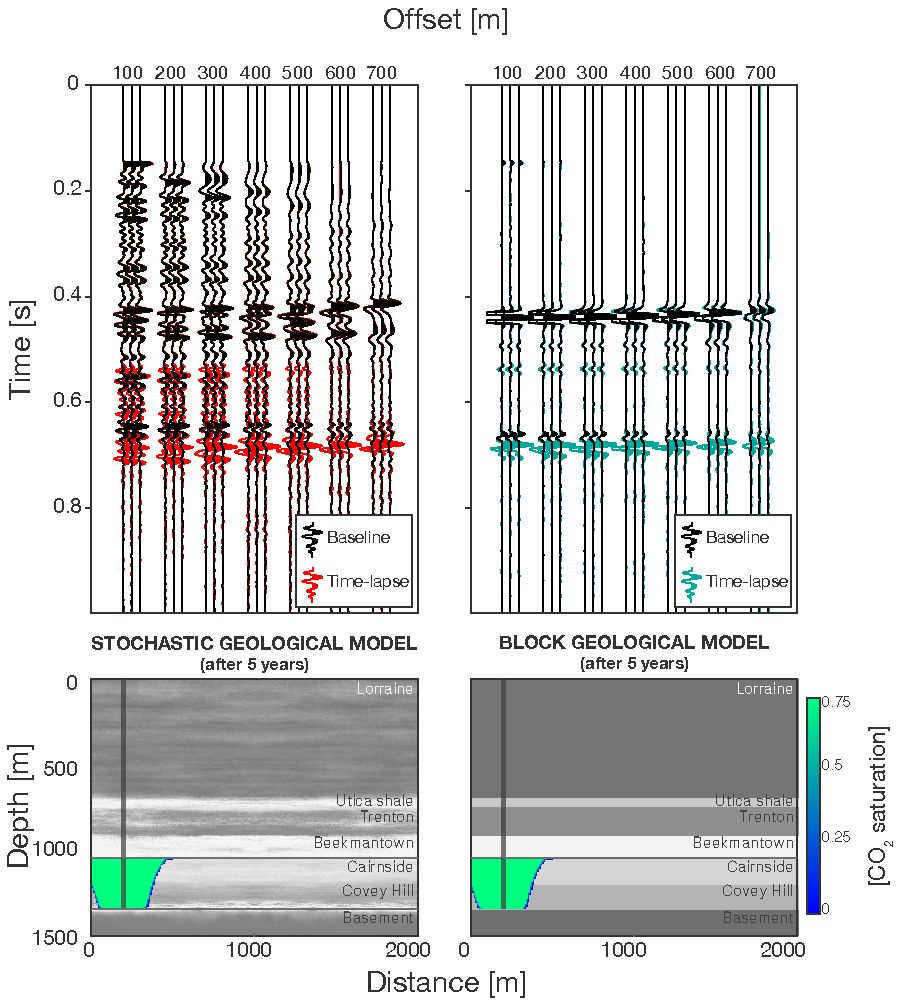
\includegraphics[width=0.9\textwidth]{fig/stochvsblock.pdf}
% \caption{Stochastic seismogram (left) versus block seismogram (right).}
% \label{fig:stochvsblock}
% \end{figure}
\begin{figure}[!ht]
        \centering
        \begin{subfigure}[b]{.5\textwidth}
                \caption{Heterogeneous model \\ (after 5 years)}
                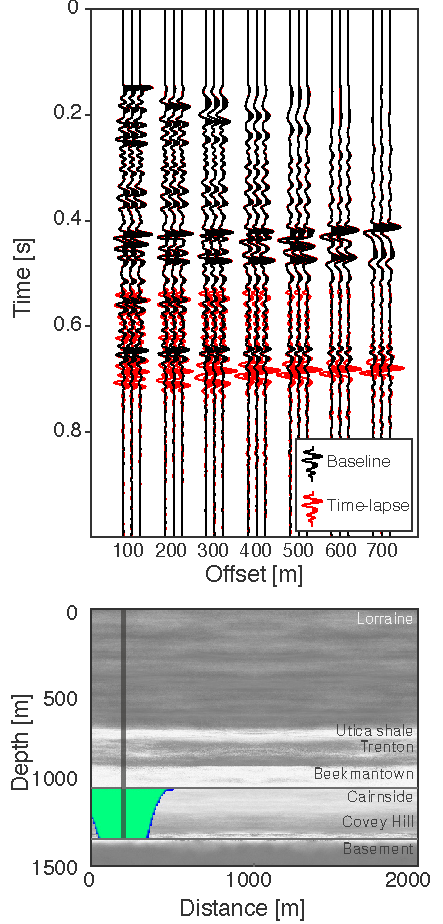
\includegraphics[width=\textwidth]{fig/stochvsblock_a.pdf}
                \label{fig:stochvsblock_a}
        \end{subfigure}%
        \begin{subfigure}[b]{.5\textwidth}
                \caption{Block model \\ (after 5 years)}
                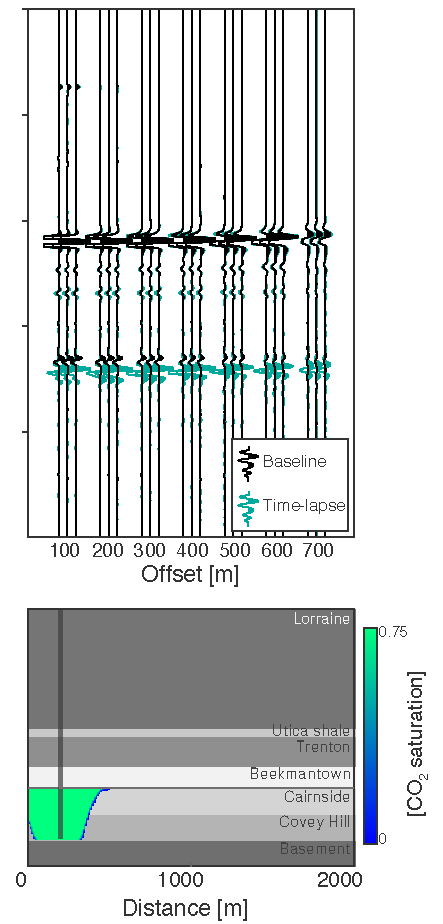
\includegraphics[width=\textwidth]{fig/stochvsblock_b.pdf}
                \label{fig:stochvsblock_b}
        \end{subfigure}
        \caption{Seismogram based on the heterogeneous model and blocky model}
        \label{fig:stochvsblock}
\end{figure}
Moreover, at the Potsdam bottom reflector, the blocky model shows an amplitude
decrease with offset. However, for the heterogeneous model, the same reflection
shows an increasing amplitude with offset. This is confirmed by the Zœppritz
analysis \citep{Aki1980} in \cref{fig:zoeppritz} where the reflection
coefficients change with the angle of incidence.
\begin{figure}[!ht]
\centering
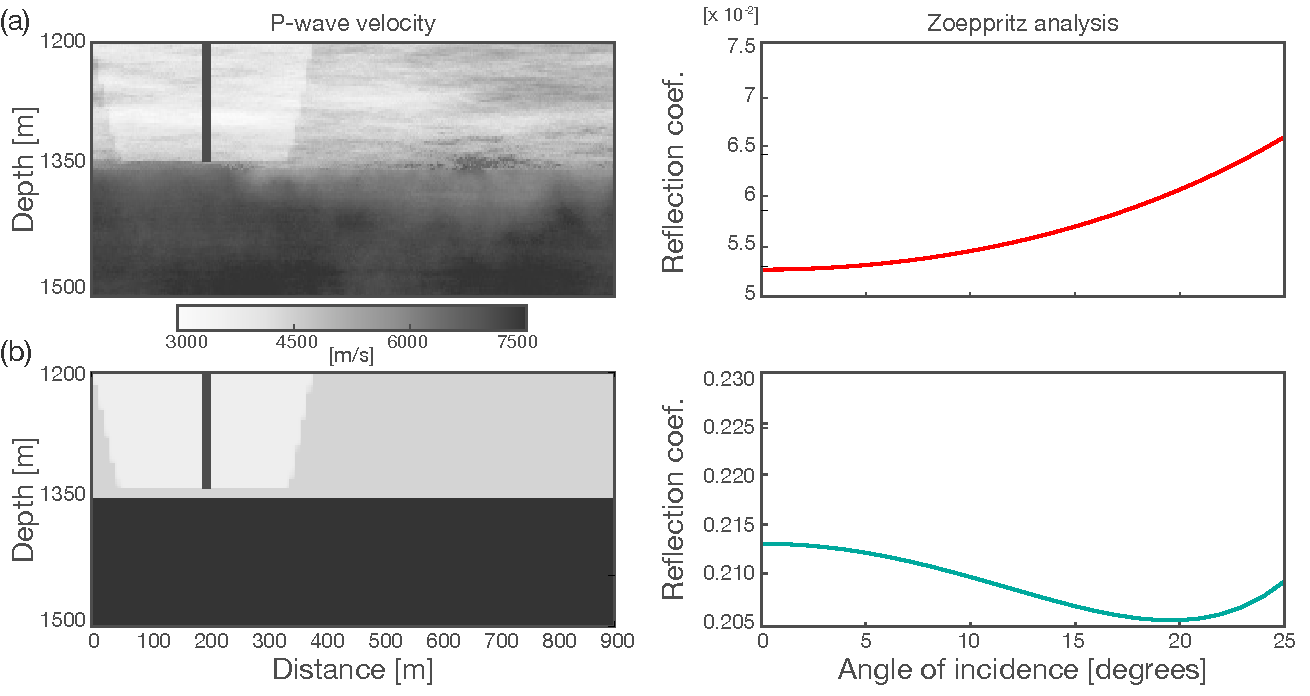
\includegraphics[width=1\textwidth]{fig/zoeppritz.pdf}
\caption{Zœppritz analysis for heterogeneous model (a) and blocky model (b)
using the CREWES Zœppritz Explorer Applet. The graphs on the right show how
reflection coefficient change with angle of incidence.}
\label{fig:zoeppritz}
\end{figure}
\section{Conclusion}
Ultrasonic measurements have been carried out on Cairnside and Covey Hill
samples of the sedimentary basin of the St.\ Lawrence Platform in southern
Quebec. The results show that $P$-waves are sensitive to pore fluid substitution
at the laboratory scale. Moreover, the measurements demonstrate that it is
possible to detect the phase transition from gaseous \ce{CO2} to liquid or
supercritical \ce{CO2}, for both velocity and amplitude attributes. \\
The laboratory measurements were used for calibrating numerical models that were
used to simulate the time-lapse seismic response to \ce{CO2} injection. A number
of scenarios were considered to evaluate the performance of a time-lapse seismic
monitoring program for the particular context of the St.\ Lawrence Platform. We
were particularly interested in comparing the response of a blocky model
(commonly used in comparable studies) with that of a model reflecting the
natural variability found in nature. We were also interested in assessing the
effect of the low permeability and porosity observed at Bécancour on the
time-lapse seismic response, and comparing the performance the seismic
monitoring with respect to more favorable storage conditions.\\
For all scenarios, a series of VSP synthetic seismograms imaging the \ce{CO2}
evolution during \num{15} years of injection and the subsequent \num{35} years
of \ce{CO2} migration have been modeled. The results show the effect of \ce{CO2}
as indicated by a time-delay of arrivals, associated with a decrease in velocity
when supercritical \ce{CO2} replaces brine in pore spaces. The geostatistical
approach used to generate our heterogeneous model allowed us to obtain more
realistic seismograms compared to a traditional blocky model. The time-lapse
amplitude response of the blocky and heterogeneous models also differ
significantly in the lower part of the reservoir.  Using over simplistic models
thus yields misleading results. It should be noted nevertheless that the
conclusions regarding the capabilities of the VSP monitoring program, as
obtained with the heterogeneous model, might be somewhat optimistic because
repeatability issues inherent to field measurements might affect its
performance.\\
For the Bécancour model, there is almost no evolution of the \ce{CO2} plume
after \num{5} years of injection and even \num{35} years after injection
stopped, and it is therefore unlikely to detect any long-term variation in the
seismic response. However, in the optimistic case the \ce{CO2} has been
partially dissolved during the migration period, and the VSP response after 50
years results in an early arrival of the reservoir bottom signal compared to the
15 years data. Therefore, carefully considering the behaviour of the reservoir
in modeling the seismic response appears critical for accurate appraisal of the
time-lapse response, which will help interpreting correctly real monitoring
data. \\
These results highlight the fact that details in the models can have significant
impacts on the expected response to a monitoring campaign. One element that was
not considered in this work are the changes in wave speeds resulting from
varying pore pressures during the injection of \ce{CO2} in the reservoir. As
reported in the literature and reiterated in the new measurements described in
this contribution, pressure effects can affect the seismic response and change
the results modeled in this study (see review in \citet{Schmitt2015}). In
particular, as pressure redistributes over time, the long-term seismic response
modeled in the Bécancour scenario should also change over time, contrary to what
is predicted without considering pressure change in the simulations.  Work is
under way to take such effects into account.
\section{Acknowledgements}
The authors would like to acknowledge E. Gloaguen for constructive comments on
an early version of the manuscript. Financial support was provided by the INRS
research chair on carbon dioxide geological storage granted by the Minist\`ere
du D\'e\-ve\-loppe\-ment durable, de l'En\-vi\-ron\-ne\-ment et des Parcs of
Qu\'ebec, as well as a research grant from Carbon Management Canada.
Computational resources were supplied by Calcul Quebec and Compute Canada.
Zœppritz analysis has been made with the Zœppritz explorer tool developed by the
Consortium for Research in Elastic Wave Exploration Seismology (CREWES).
